\documentclass[a4paper,12pt,twoside]{memoir}


% Castellano
\usepackage[spanish,es-tabla]{babel}
\selectlanguage{spanish}
\usepackage[utf8]{inputenc}
\usepackage[T1]{fontenc}
\usepackage{amsmath}
\usepackage{textcomp}
\usepackage{listings}
\usepackage{lmodern} % scalable font
\usepackage{microtype}
\usepackage{placeins}
\usepackage{tabularx}
\usepackage{adjustbox}
\usepackage{array}
\usepackage{graphicx}
\usepackage{placeins}
\usepackage{longtable}
\usepackage{ragged2e} % para \RaggedRight
\newcolumntype{P}[1]{>{\RaggedRight\arraybackslash}p{#1}}

\RequirePackage{booktabs}
\RequirePackage[table]{xcolor}
\RequirePackage{xtab}
\RequirePackage{multirow}

% Links
\PassOptionsToPackage{hyphens}{url}\usepackage[colorlinks]{hyperref}
\hypersetup{
	allcolors = {red}
}

% Ecuaciones
\usepackage{amsmath}

% Rutas de fichero / paquete
\newcommand{\ruta}[1]{{\sffamily #1}}

% Párrafos
\nonzeroparskip

% Huérfanas y viudas
\widowpenalty100000
\clubpenalty100000

% Evitar solapes en el header
\nouppercaseheads


\let\tmp\oddsidemargin
\let\oddsidemargin\evensidemargin
\let\evensidemargin\tmp
\reversemarginpar



% Imagenes
\usepackage{graphicx}
\newcommand{\imagen}[2]{
	\begin{figure}[!h]
		\centering
		\includegraphics[width=0.9\textwidth]{#1}
		\caption{#2}\label{fig:#1}
	\end{figure}
	\FloatBarrier
}






\graphicspath{ {./img/} }

% Capítulos
\chapterstyle{bianchi}
\newcommand{\capitulo}[2]{
	\setcounter{chapter}{#1}
	\setcounter{section}{0}
	\setcounter{figure}{0}
	\setcounter{table}{0}
	\chapter*{#2}
	\addcontentsline{toc}{chapter}{#2}
	\markboth{#2}{#2}
}

% Apéndices
\renewcommand{\appendixname}{Apéndice}
\renewcommand*\cftappendixname{\appendixname}

\newcommand{\apendice}[1]{
	%\renewcommand{\thechapter}{A}
	\chapter{#1}
}

\renewcommand*\cftappendixname{\appendixname\ }

% Formato de portada
\makeatletter
\usepackage{xcolor}
\newcommand{\tutor}[1]{\def\@tutor{#1}}
\newcommand{\tutorb}[1]{\def\@tutorb{#1}}
\newcommand{\course}[1]{\def\@course{#1}}
\definecolor{cpardoBox}{HTML}{E6E6FF}
\def\maketitle{
  \null
  \thispagestyle{empty}
  % Cabecera ----------------
\begin{center}
  \noindent
\includegraphics[width=\textwidth]{cabeceraSalud}\vspace{1.5cm}%
\end{center}
  
  % Título proyecto y escudo salud ----------------
  \begin{center}
    \begin{minipage}[c][1.5cm][c]{.20\textwidth}
        
\includegraphics[width=\textwidth]{escudoSalud.pdf}
    \end{minipage}
  \end{center}
  
  \begin{center}
    \colorbox{cpardoBox}{%
        \begin{minipage}{.8\textwidth}
          \vspace{.5cm}\Large
          \begin{center}
          \textbf{TFG del Grado en Ingeniería de la Salud}\vspace{.6cm}\\
          \textbf{\LARGE\@title{}}
          \end{center}
          \vspace{.2cm}
        \end{minipage}
    }%
  \end{center}
  
    % Datos de alumno, curso y tutores ------------------
  \begin{center}%
  {%
    \noindent\LARGE
    Presentado por \@author{}\\ 
    en Universidad de Burgos\\
    \vspace{0.5cm}
    \noindent\Large
    \@date{}\\
    \vspace{0.5cm}
    %Tutor: \@tutor{}\\ % comenta el que no corresponda
    Tutores: \@tutor{} -- \@tutorb{}\\
  }%
  \end{center}%
  \null
  \cleardoublepage
  }
\makeatother



% Datos de portada
\title{Segmentación automática de estructuras cerebelosas en ecografías fetales \\Documentación Técnica}
\author{Eira Rodríguez Martín}
\tutor{Pedro Latorre Carmona}
\tutorb{Roberto Martínez-Guisasola Guerrero}
\date{\today}

\begin{document}

\maketitle



\cleardoublepage



%%%%%%%%%%%%%%%%%%%%%%%%%%%%%%%%%%%%%%%%%%%%%%%%%%%%%%%%%%%%%%%%%%%%%%%%%%%%%%%%%%%%%%%%



\frontmatter

\clearpage

% Indices
\tableofcontents

\clearpage

\listoffigures

\clearpage

\listoftables

\clearpage

\mainmatter

\appendix




\apendice{Plan de Proyecto Software}

\section{Introducción}

La planificación del proyecto se ha llevado a cabo siguiendo una estructura clara, orientada a cumplir los objetivos técnicos y académicos establecidos. Todo el desarrollo y seguimiento del trabajo se ha gestionado a través del repositorio de GitHub: \href{https://github.com/eirarodriguez/fetal_brain_segmentation} {fetal\_brain\_segmentation}, donde se recoge de forma organizada la evolución del proyecto.

\section{Planificación temporal}

Para la planificación temporal del proyecto, se seleccionó GitHub Issues junto con una metodología  CRISP-DM (CRoss Industry Standard Process for Data Mining) \cite{crispdm2021}, complementada con el uso de GitHub Issues. Esta combinación permitió estructurar de forma clara tanto el desarrollo técnico como documental del proyecto, facilitando su seguimiento. El proyecto se organizó en quince sprints, con una duración de dos semanas cada uno. Dentro de cada sprint se definieron diferentes \textit{issues}, etiquetadas con \textit{labels} representativos de la fase de CRISP-DM a la que pertenece cada tarea.
 

\subsection{Sprint 1}
Fecha: 29/11/2024 - 12/11/2024

\begin{itemize}
    \item \textbf{Definición del objetivo del proyecto:} se llevaron a cabo múltiples reuniones con los tutores académicos y el obstetra. El objetivo fue comprender los requisitos clínicos, los recursos disponibles y definir el propósito central del proyecto. Durante estas sesiones se discutieron aspectos como las necesidades clínicas que el proyecto busca abordar, las imágenes disponibles y su calidad, así como las posibles limitaciones que podrían surgir.

    \item \textbf{Importación de plantilla LaTeX en Overleaf:} esta tarea consistió en la descarga de la plantilla oficial de LaTeX desde el repositorio GitHub del Grado en Ingeniería de la Salud. Posteriormente, se importó en Overleaf y se llevó a cabo una investigación sobre el uso y las funcionalidades de la herramienta para la redacción de la Memoria.
    
\end{itemize}

\subsection{Sprint 2}
Fecha: 12/11/2024 - 26/11/2024
\begin{itemize}
    \item \textbf{Documentación bibliográfica inicial:} recopilación y análisis exhaustivo de artículos científicos relacionados con la segmentación de imágenes médicas mediante \textit{deep learning}, con el fin de identificar los métodos y arquitecturas más adecuadas para el proyecto.
    \item \textbf{Redacción del documento del Comité de Ética:} esta tarea consistió en la elaboración del documento necesario para obtener la autorización y el acceso a las imágenes de ultrasonido 2D del área de Ginecología del Hospital Universitario de Burgos, esenciales para el desarrollo del proyecto. 
\end{itemize}

\subsection{Sprint 3}
Fecha: 26/11/2024 - 10/12/2024
\begin{itemize}
    \item \textbf{Redacción del documento del Comité de Ética:} continuar con el \textit{issue}. 
    \item \textbf{Revisión de imágenes proporcionadas:} antes de iniciar el procesamiento, se revisaron las imágenes ultrasonido disponibles para evaluar su calidad y observar la visibilidad de las estructuras anatómicas que se deseaban segmentar.
    \item \textbf{Evaluación de herramientas para gestión de datos anotados:} se analizaron diversas opciones de software para gestionar y explorar las imágenes y anotaciones. Inicialmente se consideró VGG Image Annotator (VIA).
    \item \textbf{Crear imagen \textit{ground truth} con VIA:} se llevó a cabo un proceso de anotación manual utilizando la herramienta VGG Image Annotator (VIA), con el objetivo de generar máscaras de referencia (\textit{ground truth}) para el entrenamiento y evaluación de los modelos de segmentación. Esta tarea consistió en delimitar con precisión las regiones anatómicas de interés en las ecografías fetales.
\end{itemize}

\subsection{Sprint 4}
Fechas: 10/12/2024 - 24/12/2024
\begin{itemize}
    \item \textbf{Revisión de imágenes proporcionadas:} continuar con el \textit{issue}.
    \item \textbf{Evaluación de herramientas para gestión de datos anotados:} continuar con el \textit{issue}.
    \item \textbf{Crear imagen \textit{ground truth} con VIA:} continuar con el \textit{issue}.
    \item \textbf{Pruebas de visualización:} se desarrolló un script en Python capaz de cargar y visualizar las imágenes de ultrasonido, adaptando su lectura al formato específico de los datos proporcionados para asegurar una correcta interpretación. La carga ha sido menor que la estimada.
    \item \textbf{Crear la máscara de las máscaras \textit{ground truth} a partir de un JSON:} a partir de los archivos generados en VIA en formato JSON, se desarrolló un script en Python que extrae las coordenadas de los polígonos anotados y asigna un color específico a cada clase según un diccionario predefinido. Como resultado, se generan máscaras segmentadas codificadas por clase, que son almacenadas en el directorio de salida para su posterior uso en el entrenamiento. La carga ha sido la estimada.
\end{itemize}   

\subsection{Sprint 5}
Fechas: 07/01/2025 - 21/01/2025
\begin{itemize}
    \item \textbf{Redacción del documento del Comité de Ética:} se realizaron modificaciones en el documento del proyecto que respondían a aclaraciones que el CEIM requería.
    \item \textbf{Implementación de métodos tradicionales de segmentación:} al inicio del proyecto se exploraron técnicas clásicas de segmentación, como \textit{K-means} y contornos activos, con el objetivo de establecer una línea de base y comprender la complejidad del problema. Sus limitaciones a la hora de capturar detalles anatómicos precisos motivaron el uso de modelos basados en aprendizaje profundo.
    \item \textbf{Investigación de técnicas de \textit{deep learning} para segmentación de imágenes:} se llevó a cabo un estudio exhaustivo sobre la aplicación de \textit{deep learning} en la segmentación de imágenes médicas.
\end{itemize}

\subsection{Sprint 6}
Fechas: 21/01/2025 - 04/02/2025
\begin{itemize}
    \item \textbf{Segmentación de \textit{deep learning} utilizando YOLOv11 y DeepLabV3+:} la primera aproximación con modelos de \textit{deep learning} incluyó la implementación de YOLOv11, adaptado para tareas de segmentación, y DeepLabV3+, conocido por su rendimiento en segmentación semántica. Sin embargo, estos modelos no ofrecieron resultados satisfactorios en el contexto del proyecto, lo que llevó a explorar arquitecturas alternativas. La carga estimada ha sido mayor a la estimada.
\end{itemize}

\subsection{Sprint 7}
Fechas:04/02/2025 - 18/02/2025
\begin{itemize}
    \item \textbf{Segmentación de \textit{deep learning} utilizando SAM:} se evaluó el modelo Segment Anything Model (SAM). Si bien SAM mostró un rendimiento aceptable en la segmentación general del cerebro, su precisión fue limitada al intentar distinguir múltiples clases específicas del cerebelo. Esto motivó la decisión de priorizar otros modelos más especializados. La carga estimada ha sido mayor a la estimada.
\end{itemize}

\subsection{Sprint 8}
Fechas: 18/02/2025 - 04/03/2025
\begin{itemize}
    \item \textbf{Evaluación de herramientas para gestión de datos anotados:} tras probar distintas arquitecturas de \textit{deep learning}, se detectó la necesidad de reorganizar los archivos de anotaciones en formato JSON. Se planteó la utilización de Roboflow, ya que permitía versionar el conjunto de datos, mantener organizadas tanto las imágenes originales como sus máscaras correspondientes, y exportar anotaciones de múltiples formatos, incluyendo COCO, que fue el seleccionado para este proyecto.
    \item \textbf{Generación de imágenes \textit{ground truth} con Roboflow:} se generaron de nuevo las imágenes \textit{ground truth} desde la plataforma de Roboflow.
    \item \textbf{Crear la máscara de las máscaras \textit{ground truth} a partir de un JSON:} con el nuevo uso de Roboflow, se genera un único archivo en formato COCO que centraliza las anotaciones de todo el conjunto de imágenes en lugar de que cada imagen, en lugar de contar con un archivo JSON por cada imagen. Esto requirió adaptar el script para recorrer el JSON global y generar las máscaras correspondientes para cada imagen.
    \item \textbf{Segmentación de \textit{deep learning} utilizando el repositorio segmentation\_models.pytorch:} tras evaluar diferentes opciones, finalmente se optó por usar la biblioteca \texttt{segmentation\_models.pytorch}, que permite implementar múltiples arquitecturas de segmentación como U-Net, U-Net++, FPN, entre otras, con una estructura de código unificada. Esta herramienta facilitó la compración entre modelos y el ajuste eficiente de hiperparámetros.
\end{itemize}
    
\subsection{Sprint 9}
Fechas: 04/03/2025 - 18/03/2025
\begin{itemize}
    \item \textbf{Segmentación de \textit{deep learning} utilizando el repositorio segmentation\_models.pytorch:} continuar con el \textit{issue}. La carga estimada ha sido mayor a la estimada.
    \item \textbf{Crear un informe sobre los resultados del proyecto:} se organizaron los resultados obtenidos tras las distintas pruebas realizadas con los modelos de segmentación. Se generó un informe inicial que cambiaría los resultados según la arquitectura con la que estuviésemos trabajando. Se incluyeron resultados visuales y cualitativos basados en los errores y aciertos del modelo. La carga estimada ha sido mayor a la estimada.
    \item \textbf{Evaluación del rendimiento de los modelos:} se analizaron diferentes métricas como la IoU (Intersection over Union) y la precisión por clase, así como un análisis visual de las máscaras segmentadas frente a la \textit{ground truth}. Este análisis permitió identificar qué arquitectura era la más adecuada para nuestro proyecto justificando su selección.
\end{itemize}

\subsection{Sprint 10}
Fechas: 18/03/2025 - 01/04/2025
\begin{itemize}
    \item \textbf{Reestructuración de las clases a segmentar:} a partir del análisis de los primeros entrenamientos, se observó un bajo rendimiento en la segmentación del cuarto ventrículo. Por ello, se optó por eliminar dicha clase y centrar el modelo en aquellas estructuras con mayor interés clínico. Además, se unificaron los hemisferios del cerebelo (inicialmente tratadas como dos clases separadas) en una sola clase, lo que contribuyó a simplificar el problema y mejorar los resultados obtenidos. La carga estimada ha sido la estimada.
    \item \textbf{Ajuste en la configuración del modelo y entrenamiento:} se realizaron ajustes iterativos en la configuración de los modelos y parámetros de entrenamiento, con el fin de maximizar el rendimiento del modelo final. La carga fue la estimada.
    \item \textbf{Crear un informe sobre los resultados del proyecto:} se repitió el \textit{issue} para cada cambio realizado.
    \item \textbf{Evaluación del rendimiento de los modelos:} se repitió el \textit{issue} para cada cambio realizado.
\end{itemize}

\subsection{Sprint 11}
Fechas: 01/04/2025 - 15/04/2025
\begin{itemize}
    \item \textbf{Implementación de \textit{data Augmentation} en el proceso de entrenamiento}: con el objetivo de enriquecer el conjunto de datos de entrenamiento y mejorar la robustez del modelo frente a variaciones en las imágenes de entrada, se implementaron técnicas de aumento de datos (\textit{data augmentation}). Esto incluyó rotaciones aleatorias, cambios de escala y ajuste de contraste, aplicadas a las imágenes durante el entrenamiento. La carga fue la estimada.
    \item \textbf{Implementación de \textit{early stopping} en el proceso de entrenamiento:} para evitar el sobreajuste, se integró la técnica de \textit{early stopping}, que permitió finalizar automáticamente el entrenamiento cuando la métrica de validación dejaba de mejorar durante varias épocas consecutivas. la carga fue menor a la estimada.
    \item \textbf{Crear un informe sobre los resultados del proyecto:} se repitió el \textit{issue} para cada técnica implementada.
    \item \textbf{Evaluación del rendimiento de los modelos:} se repitió el \textit{issue} para cada técnica implementada.
\end{itemize}

\subsection{Sprint 12}
Fechas: 15/04/2025 - 29/04/2025
\begin{itemize}
    \item \textbf{Redacción del documento del Comité de Ética:} se realizaron modificaciones en el documento del proyecto que respondían a aclaraciones que el CEIM requería.
    \item \textbf{Implementación de una aplicación:} se diseñó e implementó una interfaz gráfica sencilla utilizando la biblioteca de Streamlit, pensada para que los profesionales clínicos pudieran utilizar la segmentación sin necesidad de conocimientos técnicos. La aplicación permite cargar una imagen ecográfica y obtener la máscara segmentada de forma automática. La carga final ha sido la estimada.
    \item \textbf{Implementación de funcionalidades extra en la interfaz:} se añadieron funcionalidades adicionales, como la visualización de la \textit{ground truth} si está disponible y sus métricas, una leyenda con las clases segmentadas y la posibilidad de descargar un PDF con formato de informe médico que contiene los resultados. La carga estimada ha sido mayor a la estimada.
\end{itemize}

\subsection{Sprint 13}
Fecha: 29/04/2025 - 13/05/2025
\begin{itemize}
     \item \textbf{Subida del proyecto a GitHub:} todo el conjunto de datos, el modelo entrenado y el código de la aplicación fueron organizados y subidos al repositorio público del proyecto en GitHub. La carga final fue la estimada. 
     \item \textbf{Despliegue de la aplicación en Streamlit Community Cloud:} para permitir el acceso remoto a la aplicación sin necesidad de instalación, se publicó en Streamlit Community Cloud. Esta plataforma permite que cualquier usuario con conexión a Internet acceda a la aplicación a través del navegador, disponible en la URL: \url{https://fetalbrainsegmentation.streamlit.app/}.
     \item \textbf{Redacción de la Memoria:} elaboración del documento principal del Trabajo de Fin de Grado, que incluye la introducción del problema, los objetivos, el marco teórico, la metodología empleada los resultados obtenidos, el desarrollo de la solución propuesta, las conclusiones extraídas y las posibles líneas futuras de trabajo.
\end{itemize}

\subsection{Sprint 14}
Fechas: 13/05/2025 - 27/05/2025
\begin{itemize}
     \item \textbf{Redacción del README.md}: se redactó un archivo README.md detallado para el repositorio de GitHub. Incluye una descripción del proyecto, instrucciones de instalación y ejecución local. La carga final fue la estimada.
    \item \textbf{Redacción de anexos:} preparación y estructuración de los anexos, donde se incluirán los materiales complementarios como  la planificación, el manual para el usuario, el manual del programador, la descripción de los datos y el diseño del proyecto.
    \item \textbf{Redacción de la memoria:} continuar con la redacción de la memoria. La carga estimada ha sido mayor a la estimada.
\end{itemize}

\subsection{Sprint 15}
Fechas: 27/05/2025 - 10/06/2025
\begin{itemize}
    \item \textbf{Redacción de anexos:} continuar con la redacción de los anexos. La carga estimada ha sido mayor a la estimada.
    \item \textbf{Subir carpetas y documentos a Github}: almacenamiento en el repositorio de todo el contenido desarrollado durante el proyecto. La carga final fue la estimada.
\end{itemize}



    
\subsection{Planificación económica}
En la planificación económica se van a tener en cuenta los gastos de software, hardware y de personal, con el objetivo de proporcionar una estimación de los recursos económicos necesarios para el desarrollo del proyecto.

\subsubsection{Costes de hardware}
El desarrollo se ha realizado desde un ordenador portátil sin unidad de procesamiento gráfico (GPU) dedicada. Dada la alta demanda computacional del entrenamiento de modelos de segmentación basados en redes neuronales convolucionales, se ha optado por utilizar la plataforma Google Colab Pro que ofrece acceso a entornos con GPU.

Aunque esta opción ha sido funcional, lo adecuado para una ejecución fluida y continua de este tipo de proyectos sería disponer de un equipo con GPU dedicada. A continuación, se presentan los dos escenarios alternativos que han sido considerados para la realización de este proyecto.

\textbf{Opción A: Uso de Google Colab Pro}
A pesar de que Google Colab es una herramienta de software, se ha incluido esta opción en costes de hardware, ya que ha supuesto una alternativa a la adquisición de una GPU, que es un hardware.

Esta opción considera la amortización del equipo de trabajo principal y el coste de la suscripción a Google Colab Pro \cite{googlecolabpro_ref}. Se ha estimado el tiempo de uso en 7 meses para el portátil (duración del proyecto) y 6 meses para la suscripción, asumiendo un uso intensivo durante la fase de modelado. Los costes asociados a esta opción se resumen en la Tabla \ref{tab:costes_hardware_A}.

\begin{table}[h]
    \centering
    \begin{tabular}{@{}P{3cm} P{2.0cm} P{2.0cm} P{2.0cm} P{2.0cm}@{}}
    \textbf{Recurso} & \textbf{Precio (€)} & \textbf{Vida útil (años)} & \textbf{Tiempo de uso (meses)} & \textbf{Coste amortizado (€)} \\
    \hline
    Ordenador portátil (sin GPU)  & 900 & 5 & 7 & 105\\
    Suscripción Google Colab Pro  & 10,79 €/mes  & -- & 6 & 64,74\\
    \bottomrule
    \end{tabular}
    \caption{Costes de hardware: Uso de Google Colab Pro (Opción A).} \label{tab:costes_hardware_A}
\end{table}
\textbf{Opción B: Adquisición de equipo con GPU dedicada}
Como alternativa, se considera la adquisición de un ordenador portátil con GPU dedicada, lo que permitiría realizar los entrenamientos localmente. La amortización se calcula sobre el mismo periodo de uso. Los costes asociados a esta opción se resumen en la Tabla~\ref{tab:costes_hardware_B}.
\begin{table}[h]
    \centering
    \begin{tabular}{@{}P{3cm} P{2.0cm} P{2.0cm} P{2.0cm} P{2.0cm}@{}}
    \textbf{Recurso} & \textbf{Precio (€)} & \textbf{Vida útil (años)} & \textbf{Tiempo de uso (meses)} & \textbf{Coste amortizado (€)} \\
    \hline
    Ordenador portátil con GPU  & 1.800 & 5 & 7 & 210\\
    \bottomrule
    \end{tabular}
    \caption{Costes de hardware: Opción B (Adquisición de equipo con GPU dedicada).} \label{tab:costes_hardware_B}
\end{table}
\subsubsection{Costes de software}
Todas las herramientas utilizadas durante el desarrollo han sido gratuitas y de código abierto (ej. Python, scikit-learn, OpenCV, GitHub). Por lo tanto, no se ha incurrido en costes por licencias o suscripciones para el desarrollo. 

Para la realización de las máscaras se consideró inicialmente el uso de la versión de pago de Roboflow. Sin embargo, dado el pequeño tamaño del conjunto de datos empleado, las funcionalidades ofrecidas en su versión gratuita resultaron ser suficientes para cubrir las necesidades del proyecto.


\subsubsection{Costes de personal}
El desarrollo del proyecto ha requerido diversas tareas especializadas, incluyendo programación, procesamiento de datos, entrenamiento y evaluación de modelos de aprendizaje profundo, y despliegue de una aplicación funcional. Se estima una dedicación total de 8 meses a media jornada.

Para la estimación de los costes de personal, se ha tomado como referencia el salario medio de un ingeniero biomédico en España. Según diversas fuentes, este salario se sitúa típicamente entre los 24.000 € y 30.000 € brutos anuales. Tomando como valor representativo de 27.000 € brutos anuales \cite{glassdoor_ingenierobiomedico}, esto equivale a aproximadamente 2.250 €.

Para una dedicación a media jornada (50\% de la jornada laboral), se considera un salario mensual bruto de 1.125 €.

En la Tabla \ref{tab:costes_personal} se detallan los costes asociados al personal, incluyendo las cotizaciones a la Seguridad Social \cite{ss_cotizaciones} y retenciones de IRPF \cite{calculador_salario}, basados en una estimación promedio para un salario de esta índole en España. También se ha incluido el cálculo del coste para la empresa.
\begin{table}[h]
    \small
    \centering
    \begin{tabular}{@{}P{6cm} P{3.0cm} P{3.0cm}@{}}
    \textbf{Concepto} & \textbf{Porcentaje (\%)} &  \textbf{Coste mensual (€)} \\
    \hline
    Salario bruto  & -- & 1.125,00\\
    Retención IRPF  & 15,13\% & 170,21\\
    Cotización contingencias comunes & 4,70\% & 52,88\\
    Cotización formación  & 0,10\% & 1,13\\
    Cotización desempleo  & 1,55\% & 17,44\\
    \textbf{Total cotizaciones}  & -- & 71,45\\
    \textbf{Salario neto estimado}  & -- & 884,34\\
    \hline
    \textbf{Coste de Seguridad Social (empresa)} & -- & --\\
    Contingencias comunes (empresa) & 23,60\% & 265,50\\
    Contingencias desempleo (empresa) & 5,50\% & 61,88\\
    Contingencias formación (empresa) & 0,60\% & 6,75\\
    \textbf{Total cotizaciones (empresa)} & -- & 334,13\\
    \end{tabular}
    \caption{Costes de personal (estimación mensual).} \label{tab:costes_personal}
\end{table}

El coste total del personal se ha calculado considerando una dedicación continuada de 8 meses a media jornada de un perfil técnico con las competencias requeridas para el proyecto.

\begin{align*}
\text{Coste mensual total} &= \text{Salario bruto} + \text{Total cotizaciones (empresa)} \\
&= 1125\,\text{\texteuro{}} + 334{,}13\,\text{\texteuro{}} \\ 
&= 1459{,}13\,\text{\texteuro{}} 
\end{align*}

\begin{equation*}
\text{Coste total personal} = 1459{,}13\,\text{\texteuro{}}/\text{mes} \cdot 8 \text{meses} = 11673{,}04\,\text{\texteuro{}} 
\end{equation*}



 \subsubsection{Costes totales del proyecto}
 El coste total del proyecto se calcula sumando los costes de hardware, software y personal, para cada una de las opciones de hardware consideradas. A continuación, se muestran los costes totales estimados en función de la opción de hardware seleccionada (Tablas \ref{tab:costes_total_A} y \ref{tab:costes_total_B}).

 
 \begin{table}[h]
    \centering
    \begin{tabular}{lcc}
    \textbf{Tipo de coste} & \textbf{Coste Total}\\
    \hline
    Coste de Hardware (Opción A)  & 169,74 €\\
    Coste de Software & 0,00 €\\
    Coste de Personal & 11.673,04 €\\
    \textbf{Total} & 11.842,78 €\\
    \end{tabular}
    \caption{Costes totales del proyecto considerando la Opción A.} \label{tab:costes_total_A}
\end{table}

 \begin{table}[h]
    \centering
    \begin{tabular}{lcc}
    \textbf{Tipo de coste} & \textbf{Coste Total}\\
    \hline
    Coste de Hardware (Opción B)  & 210,00 €\\
    Coste de Software & 0,00 €\\
    Coste de Personal & 11.673,04 €\\
    \textbf{Total} & 11.883,04 €\\
    \hfill
    \end{tabular}
    \caption{Costes totales del proyecto considerando la Opción B.} \label{tab:costes_total_B}
\end{table}

\subsection{Viabilidad legal}
Los datos empleados en este proyecto consisten en ecografías 2D de cerebros fetales procedentes del Hospital Universitario de Burgos (HUBU). Al tratarse de información de pacientes, fue necesaria la aprobación por parte del  Comité de Ética de la Investigación con Medicamentos (CEIM) del HUBU. El proyecto fue aprobado el 6 de mayo de 2025, con número CEIM 3246. En la Figura \ref{fig:aprobacion_ceim} se muestra el dictamen favorable a este estudio.


\begin{figure}[h]
    \centering
    
\includegraphics[width=\textwidth]{img/ceim_aprobacion.png}
    \caption{Documento de aprobación del estudio por parte del CEIM del HUBU.}
    \label{fig:aprobacion_ceim}
\end{figure}


El desarrollo del proyecto se ha llevado a cabo conforme a la legislación vigente en materia de protección de datos y ética en investigación biomédica, incluyendo:

\begin{itemize}
    \item \textbf{Ley Orgánica 3/2018, de 5 de diciembre, de Protección de Datos Personales y garantía de los derechos digitales.}
    \item \textbf{Reglamento (UE) 2016/679 del Parlamento Europeo y del Consejo, de 27 de abril de 2016, relativo a la protección de las personas físicas en lo que respecta al tratamiento de datos personales y a la libre circulación de estos datos y por el que se deroga la Directiva 95/46/CE (Reglamento General de Protección de Datos - RGPD)}.
    \item \textbf{Ley 14/2007, de Investigación Biomédica.}
\end{itemize}
Dado que se trabaja con datos médicos sensibles (ecografías fetales), se han aplicado técnicas estrictas de anonimización para garantizar la privacidad de los participantes. Los datos proporcionados ya se encontraban codificados y no vinculados a la identidad de los pacientes, asegurando así el cumplimiento de los principios éticos y legales.


Por tanto, el proyecto se ha desarrollado dentro del marco normativo aplicable, garantizando la confidencialidad, integridad y uso ético de los datos biomédicos tratados.


\apendice{Documentación de usuario}

\section{Requisitos software y hardware para ejecutar el proyecto}

\subsection{Para el Usuario Final} 
La aplicación ha sido diseñada para ser accesible y funcional sin la necesidad de instalaciones complejas ni requisitos de hardware específicos por parte del usuario. Los requisitos de software se limitan a un navegador web, ya que la aplicación se ejecuta íntegramente en la nube. Se recomienda una conexión a Internet estable y de banda ancha para asegurar una experiencia de usuario fluida, especialmente durante la carga de imágenes para su procesamiento.

\subsection{Para el Usuario con Perfil Técnico / Investigador}
Para aquellos usuarios que precisen acceder al código fuente, realizar modificaciones, entrenar el modelo o ejecutar la aplicación localmente, se precisan los siguientes requisitos:

\begin{itemize}
    \item \textbf{Requisitos de Hardware}: Se necesita un ordenador con un procesador multinúcleo. Para un entrenamiento eficiente de modelos de \textit{deep learning}, es altamente aconsejable contar con una tarjeta gráfica (GPU) compatible con CUDA. En caso de no disponer de GPU local, se puede optar por el uso de servicios de computación en la nube con Google Colaboratory \footnote{\url{https://colab.research.google.com/}}.
    \item \textbf{Requisitos de Software}: El proyecto está desarrollado principalmente en Python. Se recomienda utilizar un gestor de entornos virtuales como \texttt{venv} para manejar las dependencias del proyecto de forma aislada. 
    
    Las bibliotecas Python necesarias están detalladas en el archivo denominado \texttt{requirements.txt} ubicado en el directorio raíz del proyecto, y pueden instalarse mediante pip. Las más destacadas incluyen:
    \begin{itemize}
        \item torch
        \item torchvision
        \item numpy, pandas, matplotlib, scikit-learn (para manipulación de datos y visualización)
        \item segmentation\_models.pytorch
        \item streamlit
    \end{itemize}
\end{itemize}
En ausencia de una GPU local, el usuario puede optar por plataformas en la nube como Google Colaboratory. Para ello, será necesario disponer de una cuenta gratuita de Google, lo que permitirá ejecutar notebooks preconfiguradas sin necesidad de instalaciones locales.


\section{Manuales y/o Demostraciones prácticas}
Esta sección describe los procedimientos necesarios para que el usuario pueda acceder y ejecutar la aplicación. 
\subsection{Para el Usuario Final}
El acceso a la aplicación para el usuario final es directo y no requiere ningún proceso de instalación. El usuario deberá abrir un navegador web y acceder a la aplicación mediante el siguiente enlace: 

\begin{center}
\url{https://fetalbrainsegmentation.streamlit.app/} 
\end{center}
 
Una vez que la página haya cargado, la interfaz principal de la aplicación estará disponible para su uso inmediato.
\subsection{Para el Usuario con Perfil Técnico / Investigador}
Para ejecutar la aplicación o las funcionalidades del proyecto localmente en otro ordenador, el usuario deberá seguir los siguientes pasos:
\begin{itemize}
    \item \textbf{Clonar el repositorio del proyecto desde GitHub}: Para obtener el código fuente del proyecto, se debe utilizar el comando en la terminal:
    
    \textbf{Nota: Es necesario tener instalado \texttt{Git} en el sistema. Puede descargarse e instalarse desde su sitio oficial web: \url{https://git-scm.com/downloads}}
    
    \begin{lstlisting}
    git clone https://github.com/eirarodriguez 
    /fetal_brain_segmentation.git
    cd fetal_brain_segmentation
    \end{lstlisting}

    \item \textbf{Instalar Python}: Se debe tener Python 3.8 o superior instalado en su sistema operativo. Se recomienda utilizar la versión más reciente compatible con las librerías del proyecto. Su descarga se puede realizar desde su sitio web oficial: \url{https://www.python.org/downloads/}
    \item \textbf{Crear un entorno virtual (opcional pero recomendado)}: Esto aísla las dependencias del proyecto del resto de su sistema Python, evitando conflictos con otras instalaciones.
    \begin{lstlisting}
    python -m venv venv
    source venv/bin/activate # En Linux/macOS
    .\venv\Scripts\activate # En Windows
    \end{lstlisting}
    \item \textbf{Instalar dependencias listadas en requirements.txt}: una vez activado el entorno virtual, instale todas las bibliotecas necesarias para el proyecto. Estas están detalladas en el archivo \texttt{requirements.txt} ubicado en la raíz del repositorio.
    \begin{lstlisting}
        pip install -r requirements.txt
    \end{lstlisting}
    \item \textbf{Ejecutar la aplicación localmente con Streamlit}: Para iniciar la interfaz de usuario web de la aplicación en su máquina local, el siguiente comando desde el directorio raíz del proyecto:
    \begin{lstlisting}
        streamlit run app.py
  \end{lstlisting}
   Esto abrirá la aplicación automáticamente en el navegador en la dirección http://localhost:8501/. Si no se abre automáticamente, el usuario puede copiar y pegar la URL que aparece en la consola en cualquier navegador web.
   \item \textbf{Ejecutar el script principal de entrenamiento}: En la carpeta \texttt{Ejemplos/} se incluyen distintos scripts de entrenamiento con configuraciones variadas. 
   
   Si se ejecuta desde Google Colab, basta con subir el notebook correspondiente en el entorno de Colab junto con el documento llamado \texttt{Informe.docx}, y ejecutar las celdas una a una. 

   En cambio, si se ejecuta desde un entorno local (por ejemplo, con Visual Studio Code), será necesario ejecutar los scripts manualmente desde la terminal. Un ejemplo sería:
   \begin{verbatim}
       python Ejemplos/early_stopping_unet.py
   \end{verbatim}
   
   Este comando ejecutará el pipeline completo: entrenamiento, evaluación del modelo y generación del informe.

    \textbf{Aclaraciones}
    Los scripts incluidos en el proyecto, están adaptados para su ejecución en Google Colab, por lo que contienen comandos específicos de dicho entorno (como \texttt{!pip install} o rutas absolutas tipo \texttt{/content/}. Si se desea ejecutarlos en un entorno local, será necesario realizar algunas adaptaciones: eliminar los comandos exclusivos de Colab y ajustar rutas de acceso a los archivos.

    Además, por motivos de protección de datos y privacidad, no se proporciona la clave API de Roboflow necesaria para descargar el proyecto. Los usuarios que deseen trabajar con un conjunto de datos deberán crear su propio conjunto de datos compatible con el formato COCO. 
   
\end{itemize}



    
     
\apendice{Manual del investigador} 

\section{Estructura de directorios}

El proyecto se entrega organizado en una carpeta principal denominada \texttt{fetal\_brain\_segmentation}, que contiene todos los archivos y subdirectorios necesarios para su ejecución y análisis. A continuación, se describe el contenido y propósito de cada uno de los elementos incluidos:

\begin{itemize}
    \item \textbf{data}: carpeta que contiene las imágenes utilizadas para el entrenamiento, validación y prueba del modelo. También incluye el archivo \texttt{\_annotations.coco.json}, que recoge las anotaciones en formato COCO utilizadas para generar las máscaras \textit{ground truth}.
    \item \textbf{Ejemplos}: contiene varios notebooks de ejemplo para el entrenamiento del modelo con diferentes configuraciones. Está organizada en tres carpetas, cada una correspondiente a una estrategia específica. En cada una se incluyen implementaciones de diferentes arquitecturas de segmentación:
    \begin{itemize}
        \item \texttt{train\_basico/}: entrenamiento técnicas adicionales, útil como línea base para comparación.
        \item \texttt{data\_augmentation/}: incluye ejemplos con técnicas de aumento de datos aplicadas para mejorar la capacidad de generalización del modelo. En esta carpeta se encuentran archivos \texttt{.py} y \texttt{.ipynb} para distintas arquitecturas.
        \item \texttt{early\_stopping/}: añade la técnica de parada temprana \textit{early stopping} a las configuraciones anteriores, con el objetivo de evitar el sobreajuste. También se organiza por arquitecturas y tipo de archivo.
    \end{itemize}
    En todas las subcarpetas se encuentran ejemplos de entrenamiento para modelos como U-Net, U-Net++, FPN, LinkNet, MANet y PSPNet.
    
    \item \textbf{Resultados}: estructurada igual que la carpeta \texttt{Ejemplos}, contiene los resultados de cada entrenamiento. Dentro de cada subcarpeta (\texttt{train\_basico}, \texttt{data\_augmentation}, \texttt{early\_stopping}) se recopilan los análisis cuantitativos (métricas como IoU y precisión) y cualitativos (visualización de segmentaciones) generados por los modelos correspondientes. Además, incluye el informe base, que contiene los marcadores utilizados para sustituir las imágenes y recoger las métricas obtenidas durante el entrenamiento.
    \item \textbf{Estado\_del\_arte}: directorio con los artículos científicos utilizados como referencia para redactar el apartado teórico del trabajo. Algunos de los artículos consultados no han podido ser descargados. 
    \item \textbf{Modelo}: Carpeta que contiene el archivo de pesos del modelo final entrenado (.pth). Este modelo es el utilizado por la aplicación de inferencia para generar las segmentaciones automáticas.
    \item \textbf{app.py}: \texit{script} principal de la aplicación desplegable mediante Streamlit. Permite cargar una imagen ecográfica, aplicar segmentación automática y mostrar los resultados junto con la máscara real si está disponible.
    \item \textbf{\texttt{LICENSE}}: archivo de licencia del proyecto, donde se especifican los términos legales de uso, modificación y distribución del código.
    \item \textbf{\texttt{README.md}}: documento de introducción al proyecto, donde se explican las instrucciones básicas de uso, instalación y ejecución.
    \item \textbf{Memoria\_TFG}: carpeta que contiene los archivos y carpetas para poder ejecutar tanto la memoria como los anexos en LaTeX. 
    \item \textbf{requirements.txt}: archivo con la lista de dependencias del proyecto. Contiene los paquetes de Python necesarios para ejecutar tanto el entrenamiento de modelos como la aplicación de inferencia. 
\end{itemize}  

\section{Compilación, instalación y ejecución del proyecto}

Los pasos necesarios para la compilación, instalación y ejecución del proyecto se encuentran detallados en el Anexo B. En él se explica cómo configurar el entorno virtual, instalar las dependencias necesarias, preparar los datos y lanzar la interfaz de usuario para realizar pruebas o usar el sistema en producción.


\section{Pruebas del sistema}

La validación del sistema se llevó a cabo mediante la supervisión directa de un profesional médico del Servicio de Ginecología y Obstetricia del HUBU. Durante el desarrollo y las fases de prueba, se le presentaron distintos ejemplos de segmentación generados por el modelo, así como una demostración completa del funcionamiento de la interfaz.

A través de observaciones cualitativas y preguntas directas, se recogió una valoración sobre la utilidad clínica del sistema, la claridad visual de los resultados y la precisión percibida en la segmentación. Esta retroalimentación resultó especialmente útil para identificar posibles mejoras desde el punto de vista del usuario final, especialmente en lo relativo a la interpretación de los datos y la usabilidad de la herramienta.



\section{Instrucciones para la modificación o mejora del proyecto}

El proyecto proporciona una base sólida para la segmentación automática de estructuras cerebrales fetales en imágenes ecográficas, y puede ser ampliado o adaptado fácilmente. A continuación, se incluyen algunas recomendaciones para facilitar su modificación o mejora por parte de futuros investigadores o desarrolladores.

El primer paso es clonar el repositorio público disponible en GitHub, el cual incluye toda la estructura de carpetas y \textit{scripts} necesarios. Se recomienda verificar las rutas de acceso a los datos, ya que pueden variar dependiendo del entorno de ejecución.

El entorno más recomendable para trabajar con el proyecto es Visual Studio Code, dada su integración con Git, soporte para Python y terminal incorporada. 

El sistema está constituido sobre PyTorch Lightning, lo cual permite una estructura clara y modular. Esto permite sustituir la arquitectura de segmentación por otra distinta, cambiar o añadir clases en el conjunto de datos, ajustar hiperparámetros e incorporar nuevas funcionalidades de pérdida o métricas de evaluación.

Estas configuraciones se pueden modificar editando las clases correspondientes en los \textit{scripts} de entrenamiento, especialmente en la clase llamada \texttt{CerebellumModelSegmentation} y en los argumentos que se le pasan.

Además, el sistema cuenta con una interfaz de usuario implementada en Streamlit, lo que permite su ejecución local de forma inmediata o su despliegue en la nube mediante plataformas como Streamlit Community Cloud. Para modificar la interfaz, basta con editar el archivo \texttt{app.py}, manteniendo la lógica principal de carga de imágenes y visualización de resultados.

En caso de entrenar un nuevo modelo, es necesario reemplazar el archivo de pesos en la carpeta correspondiente y asegurarse de que la arquitectura definida coincide con la utilizada en el \textit{script} de inferencia.

Por último, una de las principales limitaciones del proyecto es el tamaño reducido del conjunto de imágenes segmentadas manualmente. Para mejorar la precisión y generalización del modelo, se recomienda ampliar la base de datos con la colaboración de otros centros médicos u hospitales, el seguimiento longitudinal de casos en el HUBU, el uso de técnicas más avanzadas de aumento de datos y la aplicación de métodos de aprendizaje supervisado o anotación asistida.

Estas estrategias permitirían incorporar mayor diversidad gestacional, variabilidad clínica y robustez en la segmentación, incrementando así el valor clínico y la fiabilidad del sistema desarrollado.
\apendice{Descripción de la adquisición y tratamiento de datos}

\section{Descripción formal de los datos}
El conjunto de datos utilizado en este trabajo procede del Servicio de Ginecología y Obstetricia del Hospital Universitario de Burgos (HUBU). Se trata de imágenes de ecografía obstétrica 2D correspondientes al corte transversal del cerebelo fetal.

\subsection{Cohorte local}
Para el desarrollo del proyecto se planteó la utilización de un conjunto de imágenes procedentes del HUBU. La extracción de estas imágenes fue aprobada por el CEIM, en el marco del proyecto titulado "Detección de estructuras craneales en ecografías en distintas etapas del embarazo", cuyo dictamen favorable fue emitido el 6 de mayo de 2025 con número de registro CEIM 3246.

Tras su aprobación, el Servicio de Ginecología y Obstetricia del HUBU proporcionó las imágenes utilizadas en el proyecto, recopiladas en distintos periodos de tiempo. En total, se obtuvieron 198 imágenes, de las cuales 34 fueron seleccionadas como válidas para su uso en el estudio, atendiendo a criterios de calidad y adecuación anatómica.


Cada paciente incluida en el estudio había firmado un consentimiento informado firmado, y no se realizó ninguna prueba adicional con fines exclusivos de investigación. Todas las ecografías se llevaron a cabo como parte del seguimiento gestacional habitual, en el marco de atención clínica estándar.


\subsubsection{Criterios de inclusión/exclusión}
Se incluyeron en el estudio mujeres embarazadas que acudieron a la Unidad de Ecografía Fetal del Servicio de Ginecología y Obstetricia del HUBU desde el 2 de septiembre de 2024 hasta el 9 de abril de 2025, ambos incluidos, para la realización de ecografías de cribado de malformaciones fetales en diferentes semanas de gestación, y que realizaron el control gestacional completo en dicho servicio y hospital. El equipo ecográfico empleado ha de ser: Voluson E-10 de General Electric, para evitar que diferentes softwares puedan proporcionar imágenes diferentes, debido al sistema de generación de la imagen. Asimismo, se seleccionaron embarazos con progenitores de etnia caucásica, con gestaciones de origen espontáneo (sin técnicas de reproducción humana asistida), simples (un solo feto).

Quedaron excluidas del estudio aquellas mujeres embarazadas que realizaran el seguimiento del embarazo fuera del HUBU, pero que acudieron a la Unidad de Ecografía Fetal del Servicio de Ginecología y Obstetricia del HUBU para una ecografía morfológica puntual. También se excluyeron del estudio los fetos con malformación fetal mayor, o que posean marcadores de aneuploidía en ecografía de la semana 12+0 - 13+6. Además, se excluyeron aquellos progenitores cuya etnia no fuera caucásica, así como gestaciones obtenidas mediante técnicas de reproducción humana asistida o múltiples. 

\subsection{Procesamiento y anotación del conjunto de datos}

La gestión de imágenes se realizó mediante la plataforma Roboflow, que permitió:
\begin{itemize}
    \item La anotación manual precisa de las estructuras cerebelosas de interés.
    \item La creación de múltiples versiones del conjunto de datos conforme aumentaba el número de imágenes disponibles.
    \item La redimensión homogénea de las imágenes para facilitar su uso en el pipeline de entrenamiento.
    \item La exportación de las anotaciones en formato COCO, lo que facilita la integración directa en el proceso de entrenamiento y evaluación del modelo
\end{itemize}  

El conjunto final consta de 34 imágenes en formato \texttt{.jpg}, un número limitado debido a la dificultad de obtener imágenes ecográficas de alta calidad y bien anotadas. Esto justifica la segmentación manual y la puesta de bases para futuros desarrollos con conjuntos de datos más amplios. Las imágenes se distribuyen en tres subconjuntos: 26 se destinaron al entrenamiento, 4 para validación y 4 para el conjunto de prueba.

Las tres clases segmentadas son: \texttt{cerebelo} que agrupa ambos hemisferios cerebelosos, \texttt{la cisterna magna} y \texttt{vermis cerebeloso}. Esta agrupación se realizó para simplificar el modelo y reflejar la relevancia clínica de estas estructuras como unidades funcionales.

La exportación en formato COCO facilita la centralización de todas las anotaciones en un único archivo JSON estructurado, facilitando la generación automática de máscaras de segmentación.

El flujo de procesamiento del proyecto ya incluye la organización automática de los conjuntos de entrenamiento, validación y prueba.
    
\section{Descripción clínica de los datos}

El cerebelo es una de las estructuras clave en la evaluación del neurodesarrollo fetal. Su estudio en la ecografía del segundo trimestre permite detectar anomalías estructurales que pueden estar asociadas a patologías neurológicas importantes, como el síndrome de Dandy-Walker o la hipoplasia cerebelosa.

Las estructuras seleccionadas para segmentación automática tienen una relevancia directa en la evaluación clínica:

\begin{itemize}
    \item \textbf{Vermis cerebeloso:} Estructura central que conecta ambos hemisferios. Su correcta formación es clave en el control del equilibrio, la postura y la coordinación motora \cite{wolf2009vermis}.
    \item \textbf{Cisterna magna:} Ubicada bajo el cerebelo, es un espacio lleno de líquido cefalorraquídeo que juega un papel importante en la circulación del LCR y en la evaluación neuroanatómica \cite{patel2023cisternamagna}. 
    \item \textbf{Cerebelo}: compuesto por los hemisferios cerebelosos que están involucrados en la coordinación motora y el aprendizaje de movimientos \cite{volpecerebelo}.
\end{itemize}
Estas estructuras son identificadas visualmente por parte del obstetra durante el estudio ecográfico, y su segmentación automática permite facilitar y estandarizar el diagnóstico clínico.

\begin{figure}[h]
    \centering
    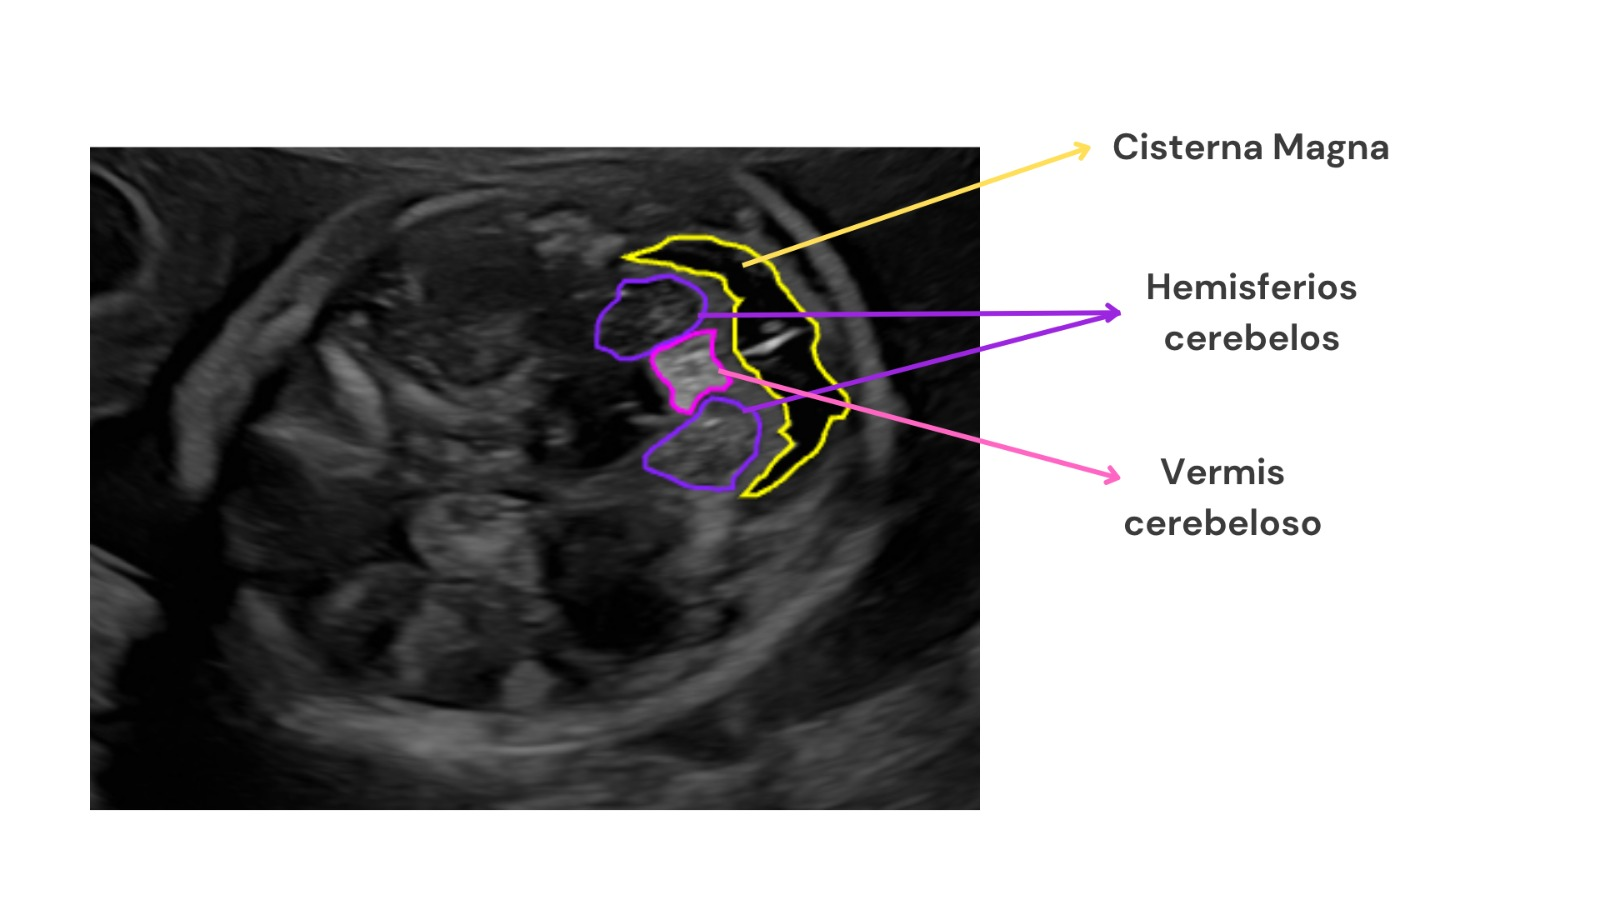
\includegraphics[width=\textwidth]{img/estructuras_interes.jpeg}
    \caption{Localización de las principales estructuras del cerebelo}
    \label{fig: parte_anatomicas_cerebelo}
\end{figure}

\apendice{Manual de especificación de diseño}

\section{Diseño arquitectónico}
Este capítulo tiene como objetivo describir la estructura interna del sistema de entrenamiento desarrollado, así como el despliegue de la interfaz gráfica, mediante el uso de diagramas explicativos que representan el flujo de trabajo del modelo de segmentación.

En la Figura \ref{fig: diagrama_de_clases} se muestra el diagrama de clases que representa los principales componentes de la fase de entrenamiento.
\begin{figure}[h]
    \centering
    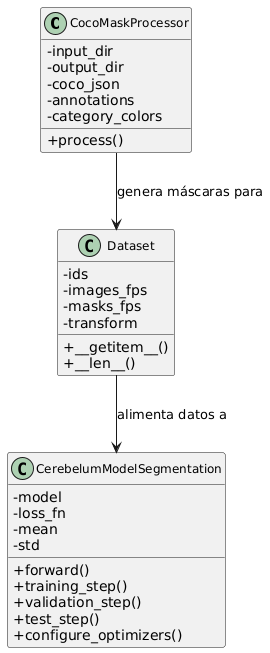
\includegraphics[width=0.5\textwidth]{img/diagrama1.png}
    \caption{Diagrama de clases del entrenamiento.}
    \label{fig: diagrama_de_clases}
\end{figure}

En la Figura \ref{fig: diagrama_interfaz} se muestra el diagrama de arquitectura funcional de la aplicación, que muestra el flujo de procesamiento desde la carga de la imagen hasta la descarga del informe en PDF, pasando por la segmentación automática y el cálculo de métricas.

\begin{figure}[h]
    \centering
    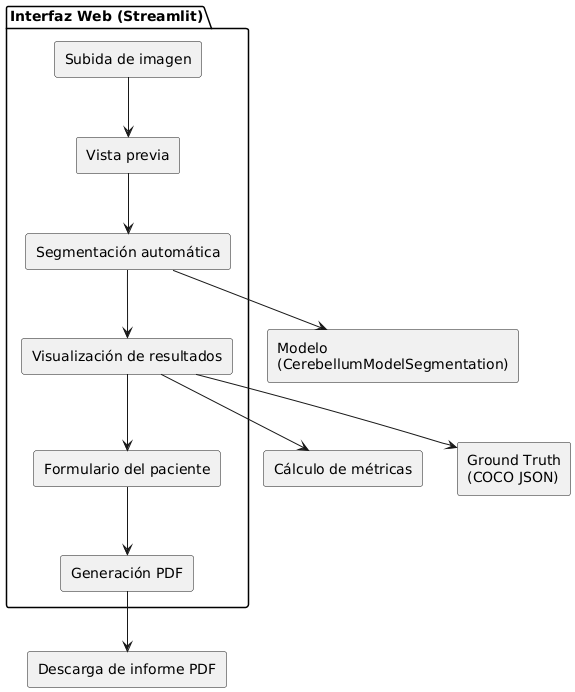
\includegraphics[width=
    \textwidth]{img/diagrama2.png}
    \caption{Arquitectura funcional de la interfaz Streamlit desarrollada.}
    \label{fig: diagrama_interfaz}
\end{figure}

\apendice{Especificación de Requisitos}


\section{Diagrama de casos de uso}
En la Figura \ref{fig: diagrama_casos_uso} se muestra el diagrama de casos de uso del sistema, diferenciando entre las funcionalidades desarrolladas por el programador y aquellas que ejecuta el médico desde la interfaz final. 
\begin{figure}[h]
    \centering
    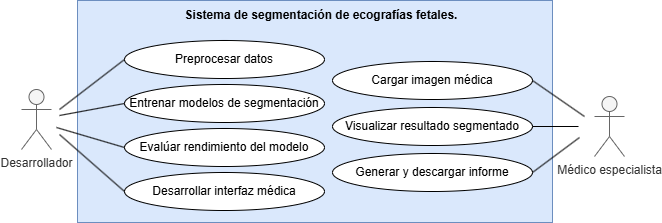
\includegraphics[width=1.1\textwidth]{img/diagrama_casos_usos.png}
    \caption{Diagrama de casos de uso.}
    \label{fig: diagrama_casos_uso}
\end{figure}

\section{Explicación casos de uso}
Esta sección presenta la explicación de los casos de uso del sistema. En cada tabla se resume de forma estructurada las principales interacciones entre los usuarios y el sistema, incluyendo su contexto, acciones implicadas y condiciones relevantes para su ejecución.

\begin{table}[!h]
	\centering
	\begin{tabularx}{\linewidth}{ p{0.21\columnwidth} p{0.71\columnwidth} }
		\toprule
		\textbf{CU-1}    & \textbf{Cargar imagen médica}\\
		\toprule
		\textbf{Versión}              & 1.0    \\
		\textbf{Autor}                & Eira Rodríguez Martín \\
		\textbf{Requisitos asociados} & RF-01 \\
        \textbf{Actor}                & Médico \\
		\textbf{Descripción}          & El usuario clínico selecciona e introduce en el sistema una imagen ecográfica fetal que será procesada para la segmentación.\\
		\textbf{Precondición}         & El usuario debe estar en la interfaz principal. \\
		\textbf{Acciones}             &
		\begin{enumerate}
			\def\labelenumi{\arabic{enumi}.}
			\tightlist
			\item El usuario hace clic en "Browse files".
			\item Se abre el explorador de archivos.
            \item El usuario selecciona una imagen valida.
            \item La imagen se carga y se muestra en la interfaz.
		\end{enumerate}\\
		\textbf{Postcondición}        & La imagen queda visible y lista para sementar. \\
		\textbf{Excepciones}          & La imagen no es válida o tiene un formato incorrecto. \\
		\textbf{Importancia}          & Alta \\
		\bottomrule
	\end{tabularx}
	\caption{CU-1 Cargar imagen médica.}
\end{table}

\begin{table}[!h]
	\centering
	\begin{tabularx}{\linewidth}{ p{0.21\columnwidth} p{0.71\columnwidth} }
		\toprule
		\textbf{CU-2}    & \textbf{Visualizar resultado segmentado}\\
		\toprule
		\textbf{Versión}              & 1.0    \\
		\textbf{Autor}                & Eira Rodríguez Martín \\
		\textbf{Requisitos asociados} & RF-02 \\
        \textbf{Actor}                & Médico \\
		\textbf{Descripción}          & El sistema genera la segmentación automática y la muestra junto a la original.\\
		\textbf{Precondición}         & Se ha cargado correctamente una imagen médica que corresponda a una ecografía del cerebro fetal. \\
		\textbf{Acciones}             &
		\begin{enumerate}
			\def\labelenumi{\arabic{enumi}.}
			\tightlist
			\item El sistema procesa automáticamente la imagen.
			\item Se ejecuta el modelo de segmentación.
            \item Se muestra el resultado en la interfaz.
		\end{enumerate}\\
		\textbf{Postcondición}        & El médico visualiza el resultado y puede interpretarlo. \\
		\textbf{Excepciones}          & Error en la predicción o visualización. \\
		\textbf{Importancia}          & Alta \\
		\bottomrule
	\end{tabularx}
	\caption{CU-2 Visualizar el resultado segmentado.}
\end{table}

\begin{table}[!h]
	\centering
	\begin{tabularx}{\linewidth}{ p{0.21\columnwidth} p{0.71\columnwidth} }
		\toprule
		\textbf{CU-3}    & \textbf{Generar y descargar el informe}\\
		\toprule
		\textbf{Versión}              & 1.0    \\
		\textbf{Autor}                & Eira Rodríguez Martín \\
		\textbf{Requisitos asociados} & RF-03 \\
        \textbf{Actor}                & Médico \\
		\textbf{Descripción}          & El sistema permite generar un informe médico en formato PDF con los resultados y datos del paciente.\\
		\textbf{Precondición}         & Debe haberse realizado la segmentación de una imagen. \\
		\textbf{Acciones}             &
		\begin{enumerate}
			\def\labelenumi{\arabic{enumi}.}
			\tightlist
			\item El usuario introduce los datos del paciente.
			\item El sistema genera el informe con la imagen original y la predicción.
            \item El usuario descarga el archivo PDF.
		\end{enumerate}\\
		\textbf{Postcondición}        & El informe queda guardado localmente. \\
		\textbf{Excepciones}          & Error al generar o guardar el archivo. \\
		\textbf{Importancia}          & Alta \\
		\bottomrule
	\end{tabularx}
	\caption{CU-3 Generar y descargar informe.}
\end{table}

\begin{table}[!h]
	\centering
	\begin{tabularx}{\linewidth}{ p{0.21\columnwidth} p{0.71\columnwidth} }
		\toprule
		\textbf{CU-4}    & \textbf{Preprocesar datos}\\
		\toprule
		\textbf{Versión}              & 1.0    \\
		\textbf{Autor}                & Eira Rodríguez Martín \\
		\textbf{Requisitos asociados} & RF-04 \\
        \textbf{Actor}                & Desarrollador \\
		\textbf{Descripción}          & El desarrollador prepara los datos de entrenamiento, generando máscaras.\\
		\textbf{Precondición}         & Disponibilidad de las imágenes. \\
		\textbf{Acciones}             &
		\begin{enumerate}
			\def\labelenumi{\arabic{enumi}.}
			\tightlist
			\item Se crean anotaciones de las imágenes.
			\item Se adaptan al formato COCO.
            \item Se generan las máscaras desde las anotaciones.
		\end{enumerate}\\
		\textbf{Postcondición}        & Los datos quedan listos para entrenar modelos. \\
		\textbf{Excepciones}          & Error en el formato de anotaciones o clases no encontradas. \\
		\textbf{Importancia}          & Alta \\
		\bottomrule
	\end{tabularx}
	\caption{CU-4 Preprocesar datos.}
\end{table}

\begin{table}[!h]
	\centering
	\begin{tabularx}{\linewidth}{ p{0.21\columnwidth} p{0.71\columnwidth} }
		\toprule
		\textbf{CU-5}    & \textbf{Entrenar modelos de segmentación}\\
		\toprule
		\textbf{Versión}              & 1.0    \\
		\textbf{Autor}                & Eira Rodríguez Martín \\
		\textbf{Requisitos asociados} & RF-05 \\
        \textbf{Actor}                & Desarrollador \\
		\textbf{Descripción}          & El desarrollador entrena modelos con los datos procesados utilizando PyTorch Lightning.\\
		\textbf{Precondición}         & Conjunto de datos preprocesado y modelo configurado. \\
		\textbf{Acciones}             &
		\begin{enumerate}
			\def\labelenumi{\arabic{enumi}.}
			\tightlist
			\item Se carga el conjunto de datos segmentado.
			\item Se define el modelo y los hiperparámetros.
            \item Se entrena con callbacks como \textit{early stopping}.
		\end{enumerate}\\
		\textbf{Postcondición}        & Modelo entrenado y guardado. \\
		\textbf{Excepciones}          & Fallos en entrenamiento. \\
		\textbf{Importancia}          & Alta \\
		\bottomrule
	\end{tabularx}
	\caption{CU-5 Entrenar modelos de segmentación.}
\end{table}

\begin{table}[!h]
	\centering
	\begin{tabularx}{\linewidth}{ p{0.21\columnwidth} p{0.71\columnwidth} }
		\toprule
		\textbf{CU-6}    & \textbf{Evaluar rendimiento del modelo}\\
		\toprule
		\textbf{Versión}              & 1.0    \\
		\textbf{Autor}                & Eira Rodríguez Martín \\
		\textbf{Requisitos asociados} & RF-06 \\
        \textbf{Actor}                & Desarrollador \\
		\textbf{Descripción}          & Evaluación del modelo con métricas como la precisión e IoU para valorar su desempeño.\\
		\textbf{Precondición}         & Modelo entrenado y conjunto de validación o prueba disponible. \\
		\textbf{Acciones}             &
		\begin{enumerate}
			\def\labelenumi{\arabic{enumi}.}
			\tightlist
			\item Se carga el modelo y los datos de evaluación.
			\item Se calculan métricas estándar de segmentación.
            \item Se comparan los resultados entre modelos entrenados.
		\end{enumerate}\\
		\textbf{Postcondición}        & Informa de métricas generado. \\
		\textbf{Excepciones}          & Métricas inconsistentes o mal calculadas. \\
		\textbf{Importancia}          & Media \\
		\bottomrule
	\end{tabularx}
	\caption{CU-6 Evaluar rendimiento del modelo.}
\end{table}



\begin{table}[!h]
	\centering
	\begin{tabularx}{\linewidth}{ p{0.21\columnwidth} p{0.71\columnwidth} }
		\toprule
		\textbf{CU-7}    & \textbf{Desarrollar interfaz médica}\\
		\toprule
		\textbf{Versión}              & 1.0    \\
		\textbf{Autor}                & Eira Rodríguez Martín \\
		\textbf{Requisitos asociados} & RF-07 \\
        \textbf{Actor}                & Desarrollador \\
		\textbf{Descripción}          & Implementación de una interfaz gráfica intuitiva que permita al médico subir imágenes, visualizar la segmentación y descargar el informe.\\
		\textbf{Precondición}         & El modelo de segmentación ya debe estar entrenado y disponible. \\
		\textbf{Acciones}             &
		\begin{enumerate}
			\def\labelenumi{\arabic{enumi}.}
			\tightlist
			\item Se diseña una interfaz adaptada al flujo clínico.
			\item Se realiza el testeo de usabilidad y funcionalidad.
		\end{enumerate}\\
		\textbf{Postcondición}        & Aplicación lista para uso clínico. \\
		\textbf{Excepciones}          & Problemas en la visualización o errores de compatibilidad. \\
		\textbf{Importancia}          & Alta \\
		\bottomrule
	\end{tabularx}
	\caption{CU-7 Desarrollar interfaz médica.}
\end{table}
\FloatBarrier
\section{Prototipos de interfaz o interacción con el proyecto}

La interfaz desarrollada para este proyecto tiene como objetivo principal facilitar el uso de la herramienta por parte del personal médico, ofreciendo una experiencia intuitiva y visualmente clara. 

En la Figura \ref{fig:subir_imagen} se muestra la forma de subir una imagen médica mediante el botón \textit{"Browse files"}.

\begin{figure}[h]
    \centering
    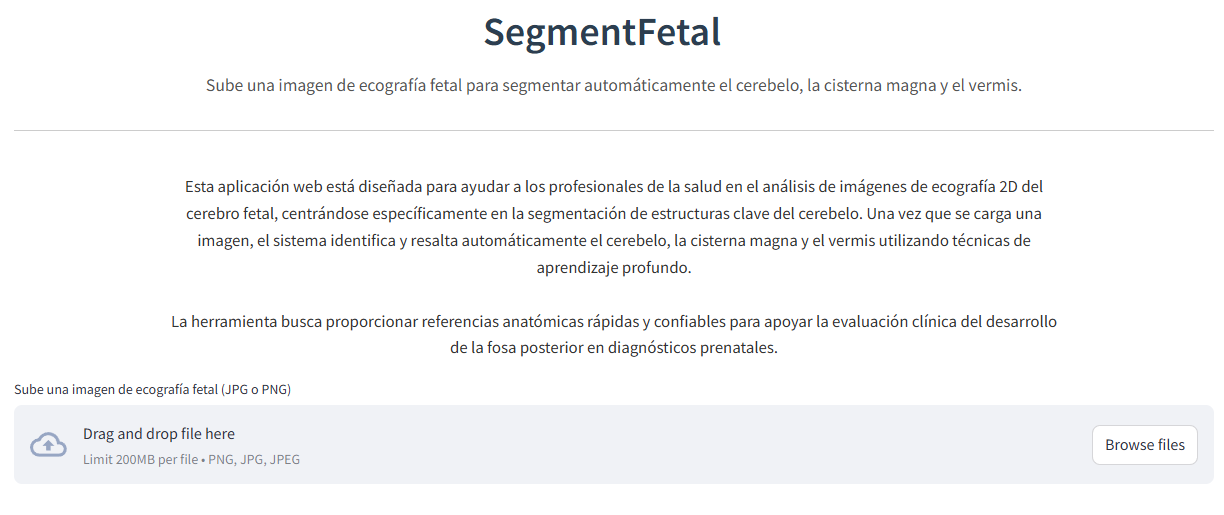
\includegraphics[width=1\textwidth]{img/interfaz_subir_imagen.png}
    \caption{Cargar imagen médica.}
    \label{fig:subir_imagen}
\end{figure}

La Figura \ref{fig:visualizar_segmentación} muestra cómo se visualizan la imagen original y la imagen tras la segmentación automática.

\begin{figure}[h]
    \centering
    \includegraphics[width=1\textwidth]{img/interfaz_visualización.png}
    \caption{Visualizar segmentación automática.}
    \label{fig:visualizar_segmentación}
\end{figure}

En la Figura \ref{fig: generar_informe} podemos observar la posibilidad de rellenar la información del paciente y generar el informe.

\begin{figure}[h]
    \centering
    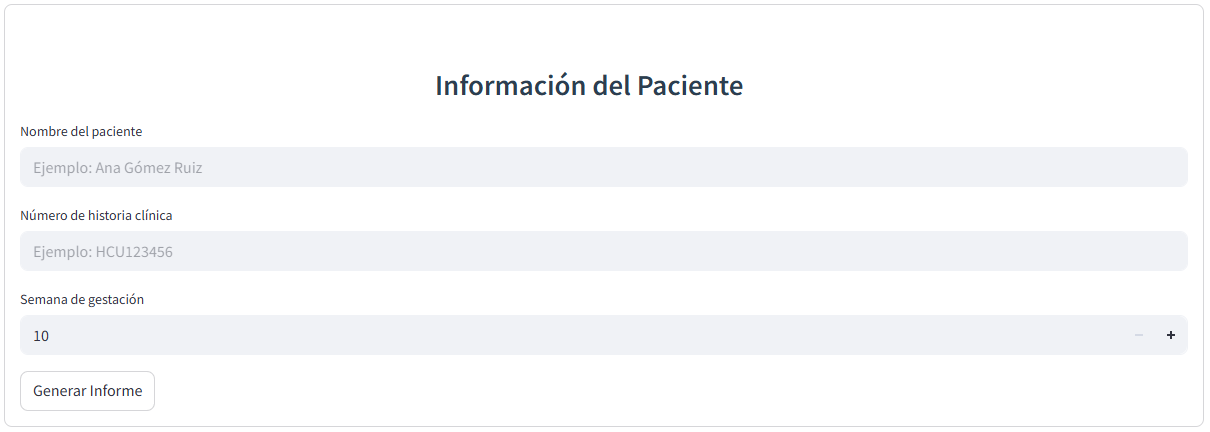
\includegraphics[width=1\textwidth]{img/interfaz_generar_informe.png}
    \caption{Generar informe.}
    \label{fig: generar_informe}
\end{figure}
\apendice{Estudio experimental}



\section{Cuaderno de trabajo}

\subsection{Comité de Ética}
El proyecto comenzó con la obtención de la aprobación ética necesaria para el uso de imágenes clínicas. Se solicitó la autorización del CEIM del HUBU para acceder a imágenes de ecografía obstétrica. 

Para ello, se redactó inicialmente un documento que describía los objetivos del estudio, la metodología y el tratamiento de los datos. Durante el proceso de evaluación, el CEIM solicitó aclaraciones y modificaciones, las cuales fueron incorporadas y respondidas puntualmente. Además, se añadieron documentos complementarios como la hoja de información al paciente y el consentimiento informado, garantizando el cumplimiento ético del estudio.

La aprobación fue concedida el 6 de mayo de 2025, con el número de registro de CEIM 3246, en el marco del proyecto titulado "Detección de estructuras craneales en ecografías en distintas etapas del embarazo". Todas las pacientes firmaron el consentimiento informado, y las imágenes utilizadas provinieron de ecografías realizadas en el seguimiento gestacional habitual, sin pruebas adicionales con fines exclusivamente investigativos.

\subsection{Primeras pruebas y modelos}

En las etapas iniciales del proyecto se exploraron diversas técnicas y modelos de segmentación de imágenes médicas con el objetivo de identificar la estrategia más adecuada para el problema clínico planteado.
\begin{itemize}
    \item \textbf{YOLOv8}: Se evaluó la viabilidad de utilizar YOLOv8 \footnote{\url{https://docs.ultralytics.com/es/tasks/segment/}}, en su variante de segmentación, un modelo desarrollado por Ultralytics que permite la segmentación en tiempo real de imágenes médicas. Sin embargo, el ruido característico de estas imágenes y la gran variabilidad entre ellas afectó negativamente a su rendimiento.
    \item \textbf{DeepLabV3+}: También se probaron modelos basados en la arquitectura DeepLabV3+, reconocida por su eficacia. No obstante, sus resultados no fueron suficientemente precisos para tareas de segmentación detallada.
    \item \textbf{Segment Anything Model (SAM)}: Se utilizó SAM para integrar una segmentación inicial del contorno cerebral, con el objetivo posterior de aplicar una segmentación más fina sobre las estructuras internas. Sin embargo, los resultados tampoco fueron satisfactorios debido a la naturaleza borrosa y variable de las ecografías fetales.
\end{itemize}
Por último, se optó por utilizar la librería \texttt{segmentation\_models\_pytorch}, que ofrece la implementación de un mismo modelo para el uso de varias arquitecturas como \texttt{Unet}, \texttt{Unet++}, \texttt{Linknet}, \texttt{FPN}, \texttt{MAnet}, \texttt{PSPNet} basados en redes convolucionales profundas. Esta elección permitió obtener una mayor precisión.

\subsection{Desarrollo de la aplicación local}
Una vez entrenado el modelo y almacenado el mejor resultado mediante la funcionalidad de \texttt{checkpoints}, utilizando el conjunto de datos clínicos obtenido del HUBU, se procedió al desarrollo de una aplicación local con el objetivo de facilitar su uso por parte del personal clínico.

La aplicación fue desarrollada con \textit{Streamlit}, una biblioteca de Python que permite la creación de interfaces gráficas de manera sencilla. La versión inicial permitía cargar imágenes de ecografía y visualizar las predicciones de segmentación generadas por el modelo.

Posteriormente, tras recibir sugerencias del profesional médico colaborador, se incorporaron funcionalidades adicionales, como la visualización de la máscara \textit{ground truth} (cuando estaba disponible) y la generación automática de informes en formato PDF con los resultados obtenidos.

Esta aplicación local permitió ajustar la interfaz en función del uso clínico, situando cada elemento en la disposición más adecuada para una experiencia intuitiva y centrada en el usuario.

\subsection{Proceso de despliegue a la nube}
Para el acceso remoto a la herramienta, el modelo fue desplegado en la nube. Para ello, tanto los datos como el modelo y el código fueron subidos al repositorio de GitHub del proyecto \href{https://github.com/eirarodriguez/fetal_brain_segmentation} {fetal\_brain\_segmentation}. 

Posteriormente, utilizando la plataforma \textit{Streamlit Community Cloud}, que permite la ejecución directa del código desde un repositorio, se generó una URL pública que permite el acceso a la aplicación sin necesidad de instalación local, facilitando así su evaluación y uso desde cualquier ubicación.


\subsection{Validación del personal clínico} 
Se contó con la colaboración de un profesional médico de la unidad de obstetricia, quien participó activamente en la validación de cada una de las etapas del proyecto.

Para validar el modelo de segmentación, se le enviaron los informes generados automáticamente con los resultados obtenidos por cada arquitectura evaluada. 

Además, se le consultó sobre la relevancia clínica para segmentar el cuarto ventrículo, estructura que inicialmente formaba parte del conjunto de clases, para cuya detección resultó poco consistente debido a su pequeño tamaño. Tras su evaluación, se concluyó que no era esencial para el propósito clínico del proyecto, por lo que se decidió centrar la segmentación en estructuras de mayor importancia.

Una vez desarrollada la aplicación, se enviaron al profesional videos explicativos sobre su funcionamiento. Finalmente, tras incorporar todas las funcionalidades propuestas, se compartió la URL de la versión desplegada, la cual fue revisada y se considera satisfactoria para su uso.

\section{Configuración y parametrización de las técnicas}

Durante el desarrollo del modelo de segmentación, se ajustaron progresivamente los parámetros y la configuración del entrenamiento con el objetivo de mejorar la precisión sin comprometer la eficiencia computacional ni el cumplimiento clínico del proyecto.

\subsection{Arquitectura y encoder} 

La arquitectura seleccionada fue \texttt{U-Net}, con el encoder \texttt{ResNeXt50\_32x4d}, preentrenado en ImageNet. Esta combinación demostró un rendimiento sólido en las pruebas realizadas en el conjunto clínico disponible.

\subsection{Función de pérdida}
Para la optimización del modelo se utilizó la función de pérdida \texttt{DiceLoss} en modo \texttt{multiclass}. Esta función está basada en el coeficiente Dice, una métrica que cuantifica la similitud entre dos conjuntos, en este caso, la máscara predicha y la máscara de referencia.

También fue configurada para trabajar directamente con los \textit{logits} del modelo, permitiendo una optimización directa y estable desde el inicio del entrenamiento.

\subsection{Parámetros de entrenamiento}
Los parámetros de entrenamiento se definieron a partir de configuraciones base ampliamente utilizadas en segmentación multiclase con redes convolucionales profundas, partiendo del código de la comunidad oficial de \texttt{segmentation\_models\_pytorch}. Posteriormente, fueron ajustados para adaptarse a las particularidades de las imágenes clínicas en este proyecto.
\begin{itemize}
    \item \textbf{Épocas (\texttt{max\_epochs})}: se estableció un límite de 200 épocas como máximo. Este valor alto permite al modelo un entrenamiento profundo, pero se controló mediante \textit{early stopping} para evitar el sobreajuste, deteniendo el proceso automáticamente si la pérdida no mejoraba en 30 épocas consecutivas. 
    \item \textbf{Tamaño del batch (\texttt{Batch size})}: se utilizó un batch size de 1, lo cual es común en tareas de segmentación médica, especialmente cuando se trabaja con imágenes grandes o cuando se dispone de recursos computacionales limitados. Esta configuración permite mantener la carga de memoria dentro de los límites de la GPU utilizada.
    \item \textbf{Optimizador (Adam)}: se seleccionó el optimizador \texttt{Adam}, ampliamente adoptado en redes neuronales profundas. Su principal ventaja es que adapta la tasa de aprendizaje de forma individual para cada parámetro, lo que la hace especialmente útil en escenarios con ruido o desbalances entre clases, como lo son las ecografías médicas.
    \item \textbf{Tasa de aprendizaje (\texttt{learning rate})}: se estableció un valor inicial de 0,0002. Este valor moderadamente bajo favorece una convergencia estable, especialmente en los primeros pasos del entrenamiento. 
    \item \textbf{Scheduler}: se aplicó un scheduler de tipo coseno, configurado con un valor mínimo de tasa de aprendizaje de 0,00001 y un ciclo de 50 épocas. Esta estrategia ayuda a refinar los pesos del modelo en fases avanzadas del entrenamiento, evitando que quede atrapado en mínimos poco óptimos.
\end{itemize}
\subsection{Callbacks de entrenamiento}
\begin{itemize}
    \item \textbf{Early stopping}: se utilizó con una paciencia de 30 épocas, monitorizando la pérdida de validación. Esta estrategia permitió evitar sobreajuste y reducir el tiempo de entrenamiento.
     \item \textbf{Model checkpoint}: se guardó automáticamente el modelo con la menor pérdida de validación registrada durante el entrenamiento, facilitando su posterior evaluación y despliegue.
\end{itemize}
\subsection{Augmentaciones y reprocesamiento}
Para mejorar la capacidad de generalización del modelo, se aplicaron técnicas de \textit{data aumentation} durante el entrenamiento, incluyendo rotaciones, desplazamientos, ajustes de brillo y contraste, así como normalización. Durante la validación y prueba, se utilizó únicamente la normalización estándar.

\section{Detalle de resultados}
En la carpeta de Resultados, disponible en el repositorio de GitHub del proyecto, se incluyeron los informes generados sobre el conjunto de prueba. Cada informe contiene:
\begin{itemize}
    \item Cuatro imágenes de prueba, con su \textit{ground truth} y la segmentación predicha por el modelo.
    \item Una tabla con métricas por clase (precisión e IoU).
    \item El promedio de estas métricas para cada imagen.
    \item La evolución de la función de pérdida durante el entrenamiento.
\end{itemize}

Estos elementos permitieron realizar una evaluación tanto cuantitativa como cualitativa del comportamiento de cada modelo.

En la Tabla \ref{tab:resultados_earlystopping}, se presenta una comparativa de métricas medias para arquitectura. Los resultados se obtuvieron aplicando técnicas de \textit{data augmentation} y \textit{early stopping} durante el entrenamiento, y fueron evaluados sobre el conjunto de prueba. 

\begin{table}[h]
    \centering
    \begin{tabular}{lcc}
    \textbf{Arquitectura} & \textbf{Precisión media (\%)} & \textbf{IoU media (\%)} \\
    \hline
    U-Net             & 70,74 & 63,69\\
    U-Net++           & 67,07 & 62,46\\
    FPN               & 70,77 & 60,23\\
    PSPNet            & 15,06 & 12,11\\
    LinkNet           & 71,12 & 60,32\\
    MAnet             & 61,49 & 55,62\\
    \hfill
    \end{tabular}
    \caption{Comparativa de métricas medias por arquitectura sobre el conjunto de prueba con \textit{early stopping}.} \label{tab:resultados_earlystopping}
\end{table}

El modelo U-Net alcanzó una IoU media del 63,69\%, lo que confirma su capacidad para segmentar con precisión estructuras cerebrales en ecografías obstétricas, superando consistentemente a otras arquitecturas evaluadas. Este valor se considera adecuado dentro del contexto clínico del proyecto, donde una IoU superior al 60\% permite una interpretación fiable por parte del personal médico.

Entre todos los modelos evaluados, U-Net obtuvo el mejor rendimiento en términos de IoU media, lo que respalda su elección como arquitectura base en tareas de segmentación médica. Sin embargo, U-Net++ y LinkNet también presentaron resultados competitivos, ligeramente por debajo.

Por el contrario, PSPNet mostró un rendimiento significativamente inferior, lo que evidencia su inadecuación para este tipo de imágenes, posiblemente debido a su diseño más orientado a escenas urbanas complejas y no a estructuras anatómicas.

A partir de esta comparativa, se seleccionaron tres arquitecturas representativas para un análisis más detallado:

\begin{itemize}
    \item \textbf{U-Net}: como referencia estándar, por ser la arquitectura con mayor IoU media y comportamiento robusto.
    \item \textbf{LinkNet}: por su precisión competitiva y eficiencia computacional.
    \item \textbf{PSPNet}: como ejemplo de arquitectura menos adecuada, dada su baja precisión y capacidad de segmentación en este dominio.
\end{itemize}

En las Figuras \ref{fig:comparacion_unet}, \ref{fig:comparacion_linknet} y \ref{fig:comparacion_pspnet}, se muestran visualizaciones de las predicciones generadas por estas tres arquitecturas, comparando la imagen original, la máscara real y la predicción del modelo.

\begin{figure}[h]
    \centering
    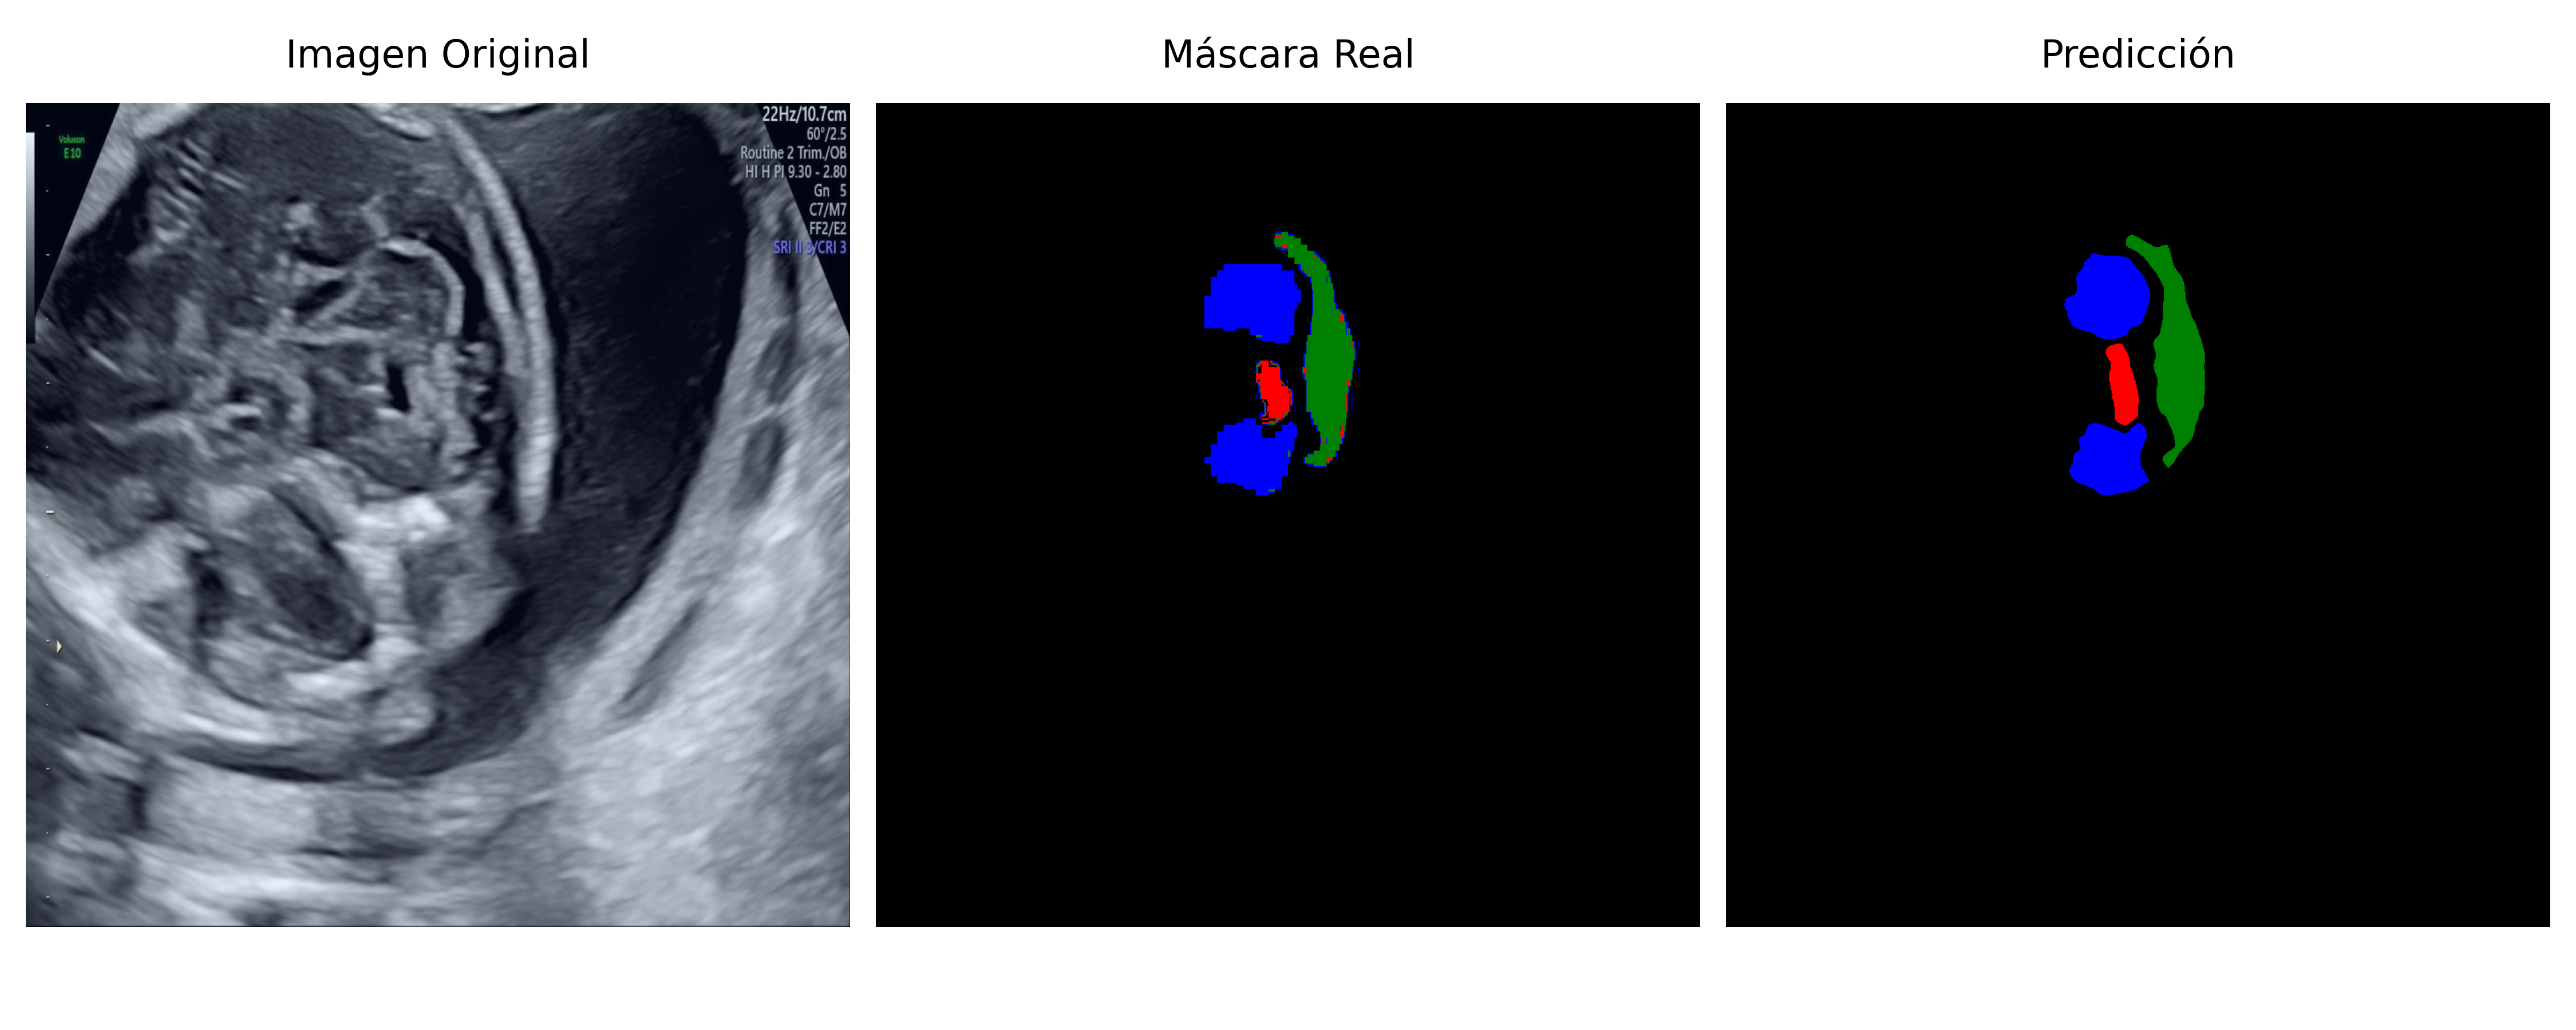
\includegraphics[width=1\textwidth]{img/image1_unet.png}
    \caption{Comparación visual de la segmentación generada por U-Net. De izquierda a derecha: imagen original, \textit{ground truth}, predicción del modelo. }
    \label{fig:comparacion_unet}
\end{figure}

\begin{figure}[h]
    \centering
    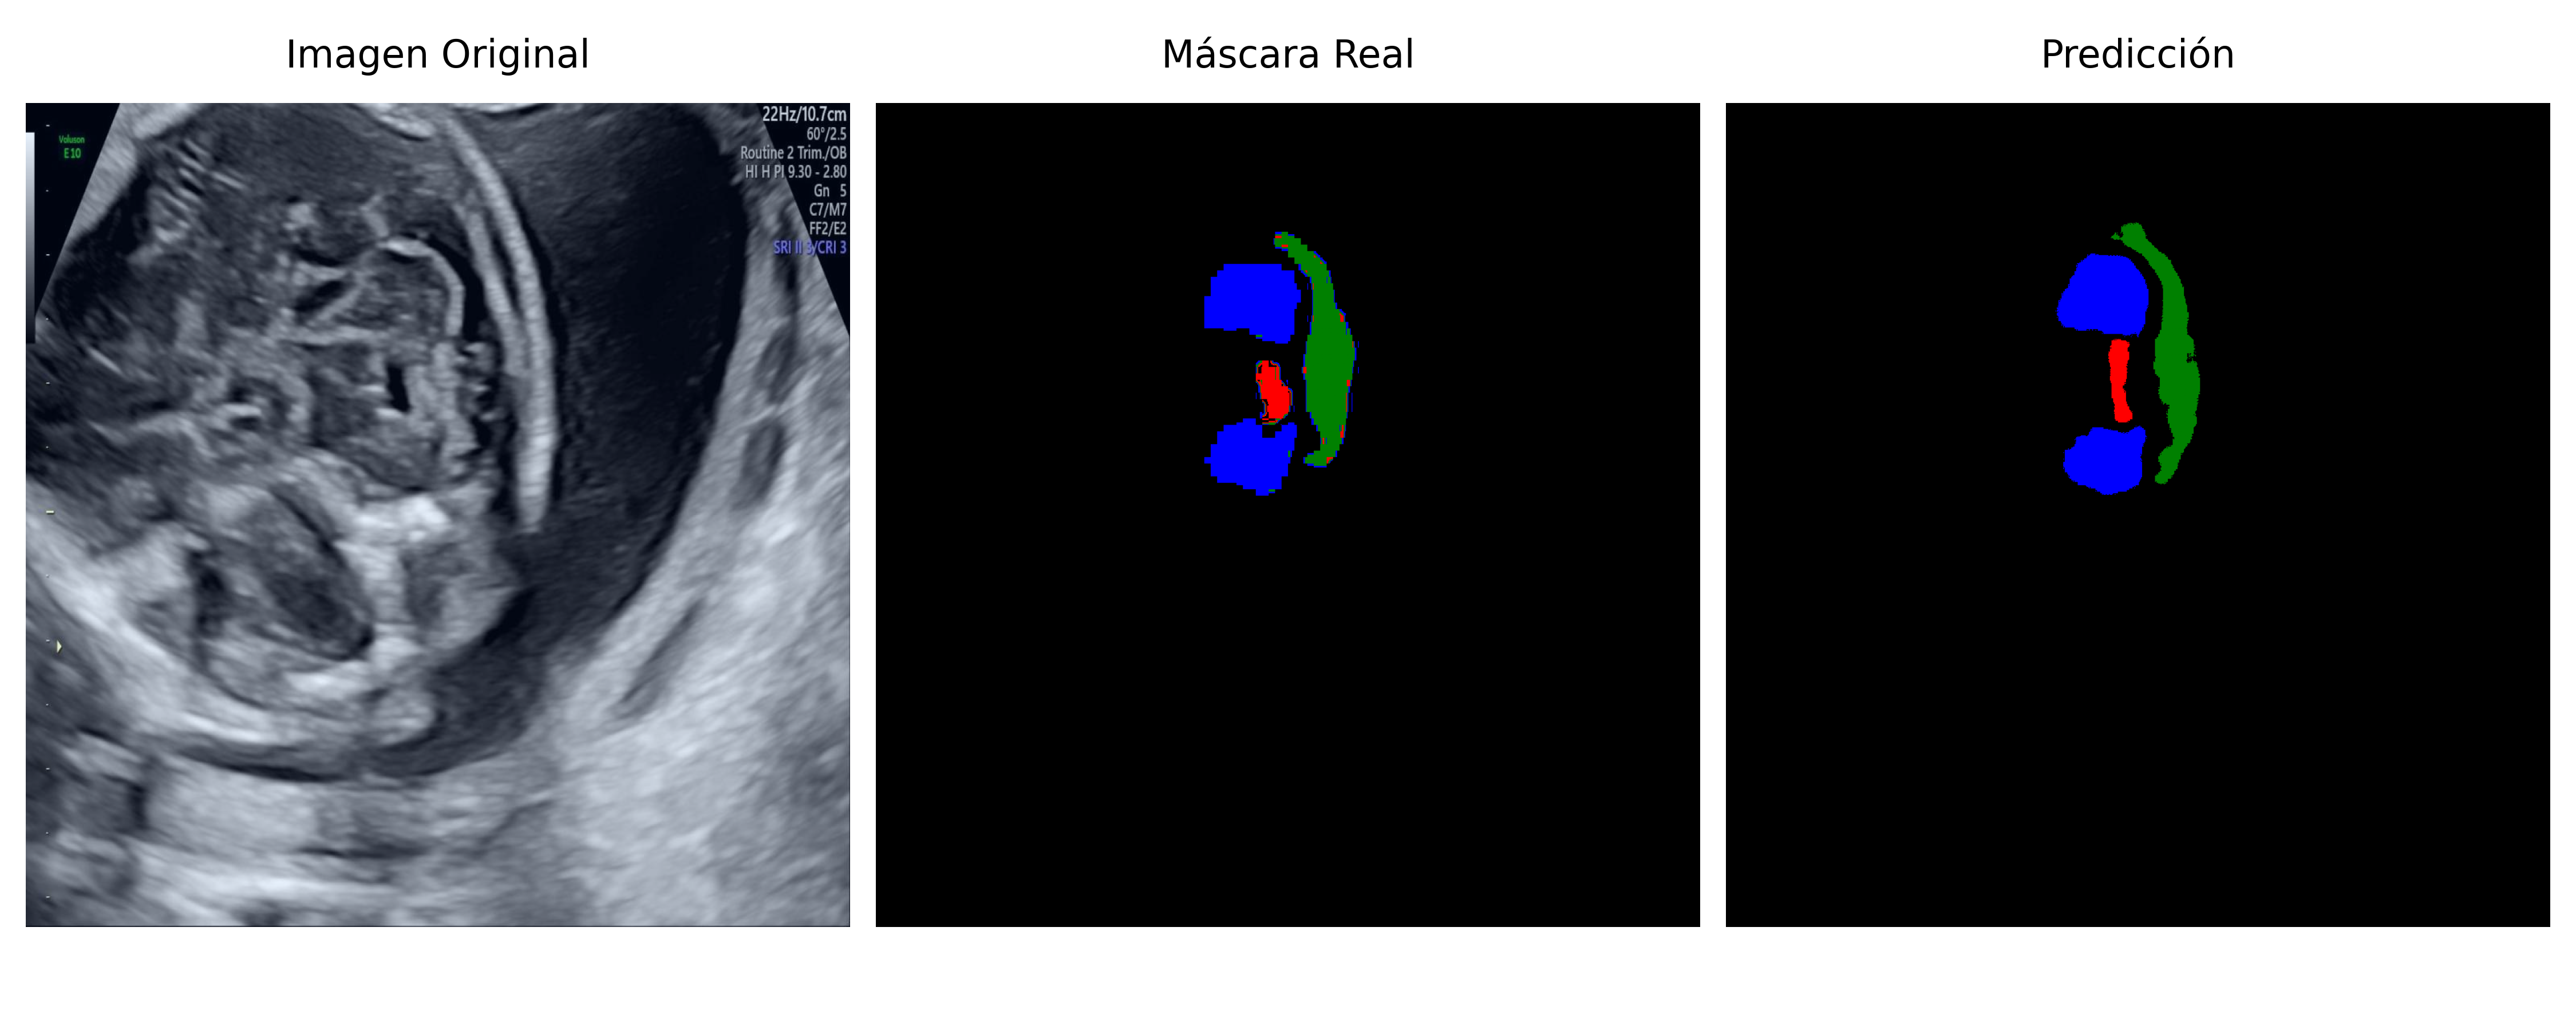
\includegraphics[width=1\textwidth]{img/image1_linknet.png}
    \caption{Comparación visual de la segmentación generada por LinkNet. De izquierda a derecha: imagen original, \textit{ground truth}, predicción del modelo.}
    \label{fig:comparacion_linknet}
\end{figure}

\begin{figure}[h]
    \centering
    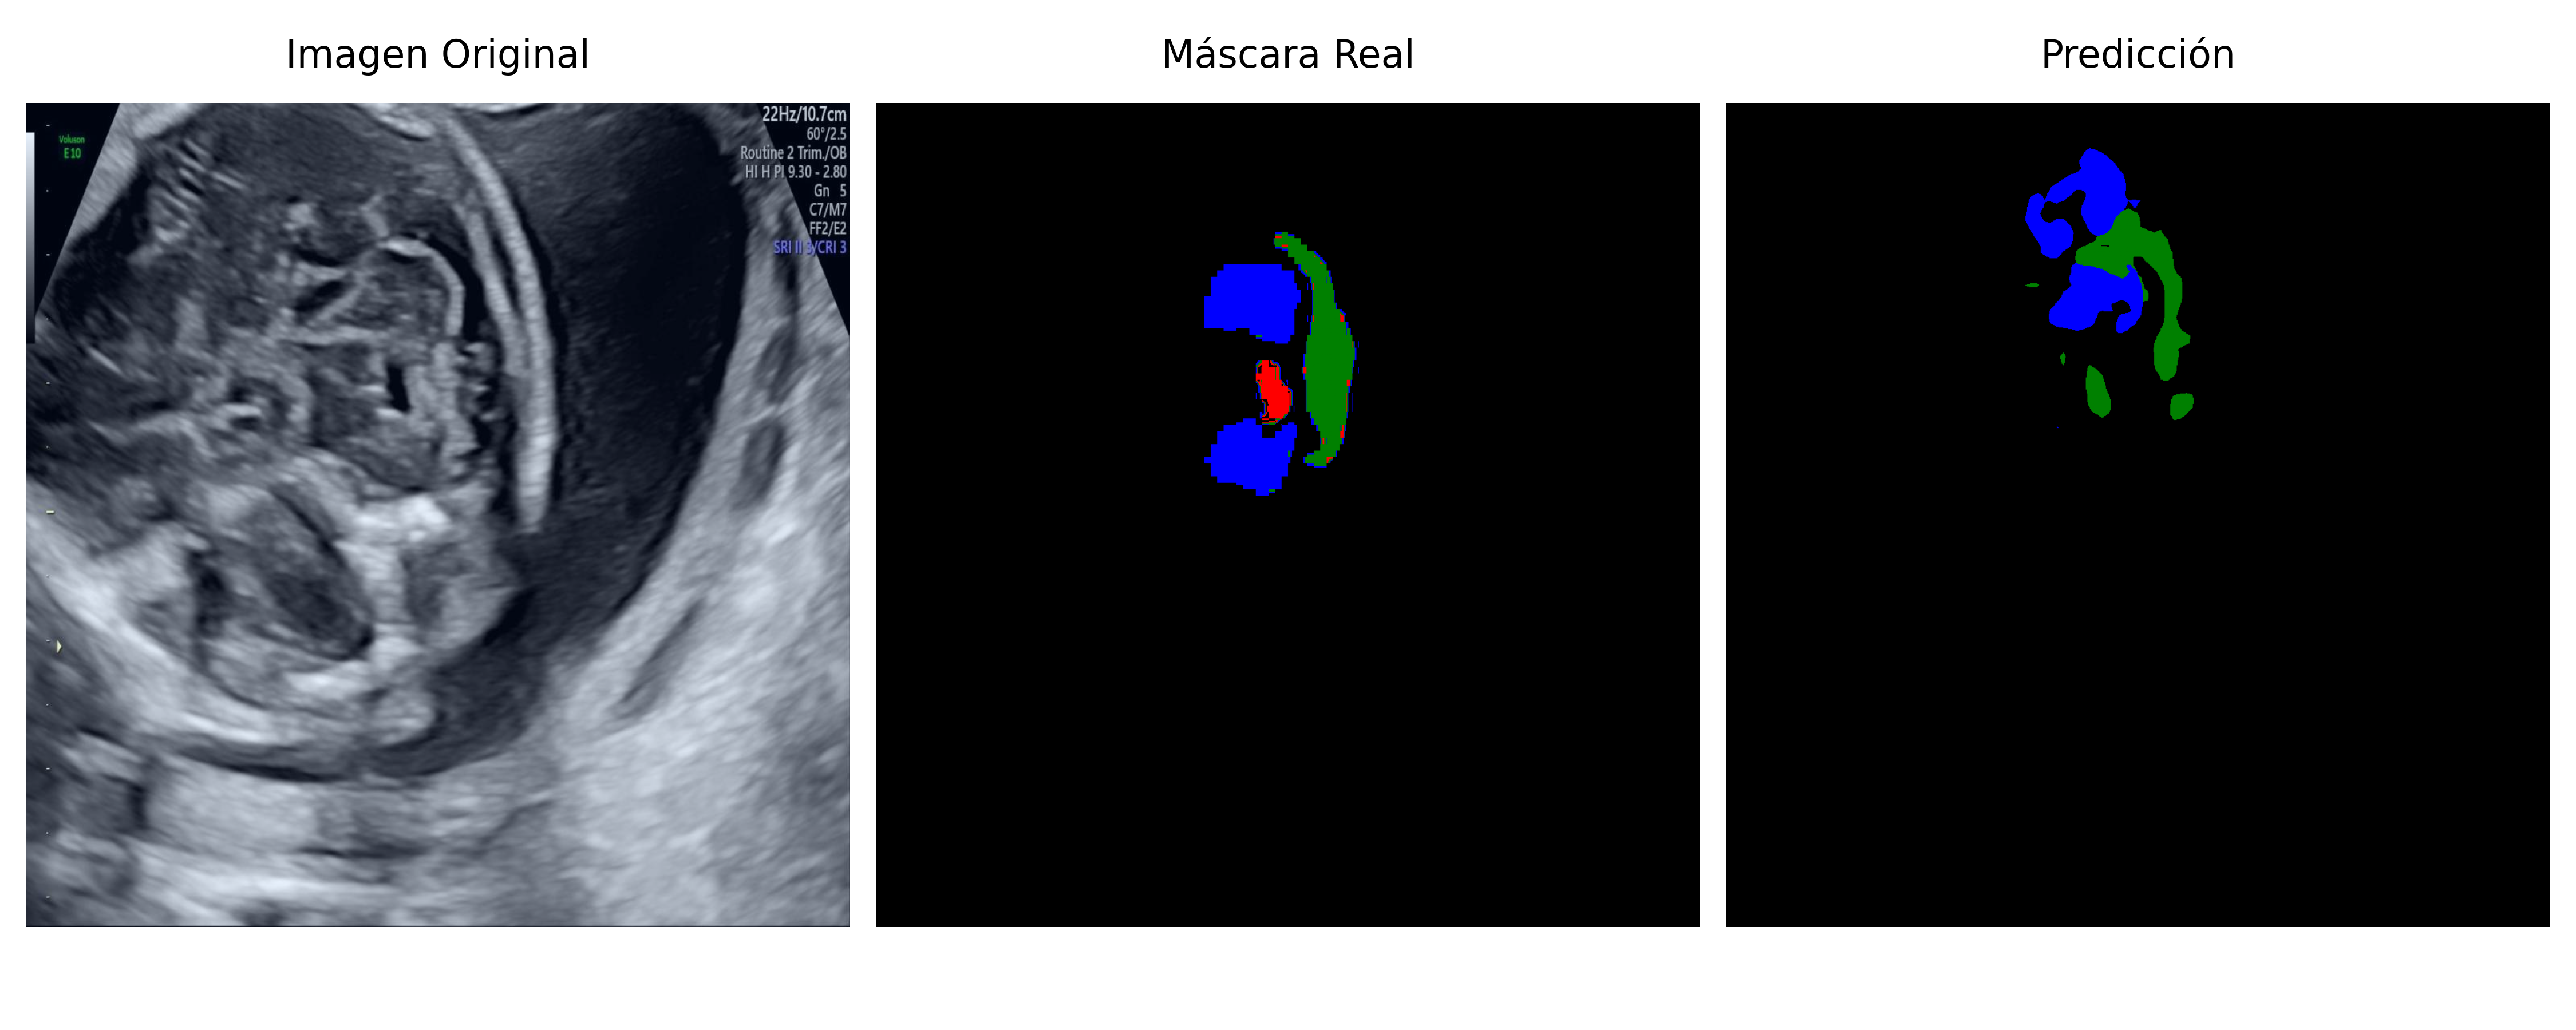
\includegraphics[width=1\textwidth]{img/image1_pspnet.png}
    \caption{Comparación visual de la segmentación generada por PSPNet. De izquierda a derecha: imagen original, \textit{ground truth}, predicción del modelo.}
    \label{fig:comparacion_pspnet}
\end{figure}

Estas comparaciones permiten identificar las diferencias en el comportamiento de cada red. Mientras que U-Net consigue representar con bastante fiabilidad las estructuras del cerebelo, PSPNet falla al captar los entornos y tiende a subsegmentar o ignorar regiones relevantes.

Con base en este análisis, se optó por utilizar U-Net como modelo principal para la interfaz final, debido a su mayor IoU media y a la calidad de sus predicciones visuales.

Las visualizaciones adicionales incluidas en las Figuras \ref{fig:comparacion_unet2}, \ref{fig:comparacion_unet3} y \ref{fig:comparacion_unet4} respaldan el buen desempeño de U-Net, mostrando una segmentación consistente y adaptada a las variaciones presentes en las imágenes ecográficas.

\begin{figure}[h]
    \centering
    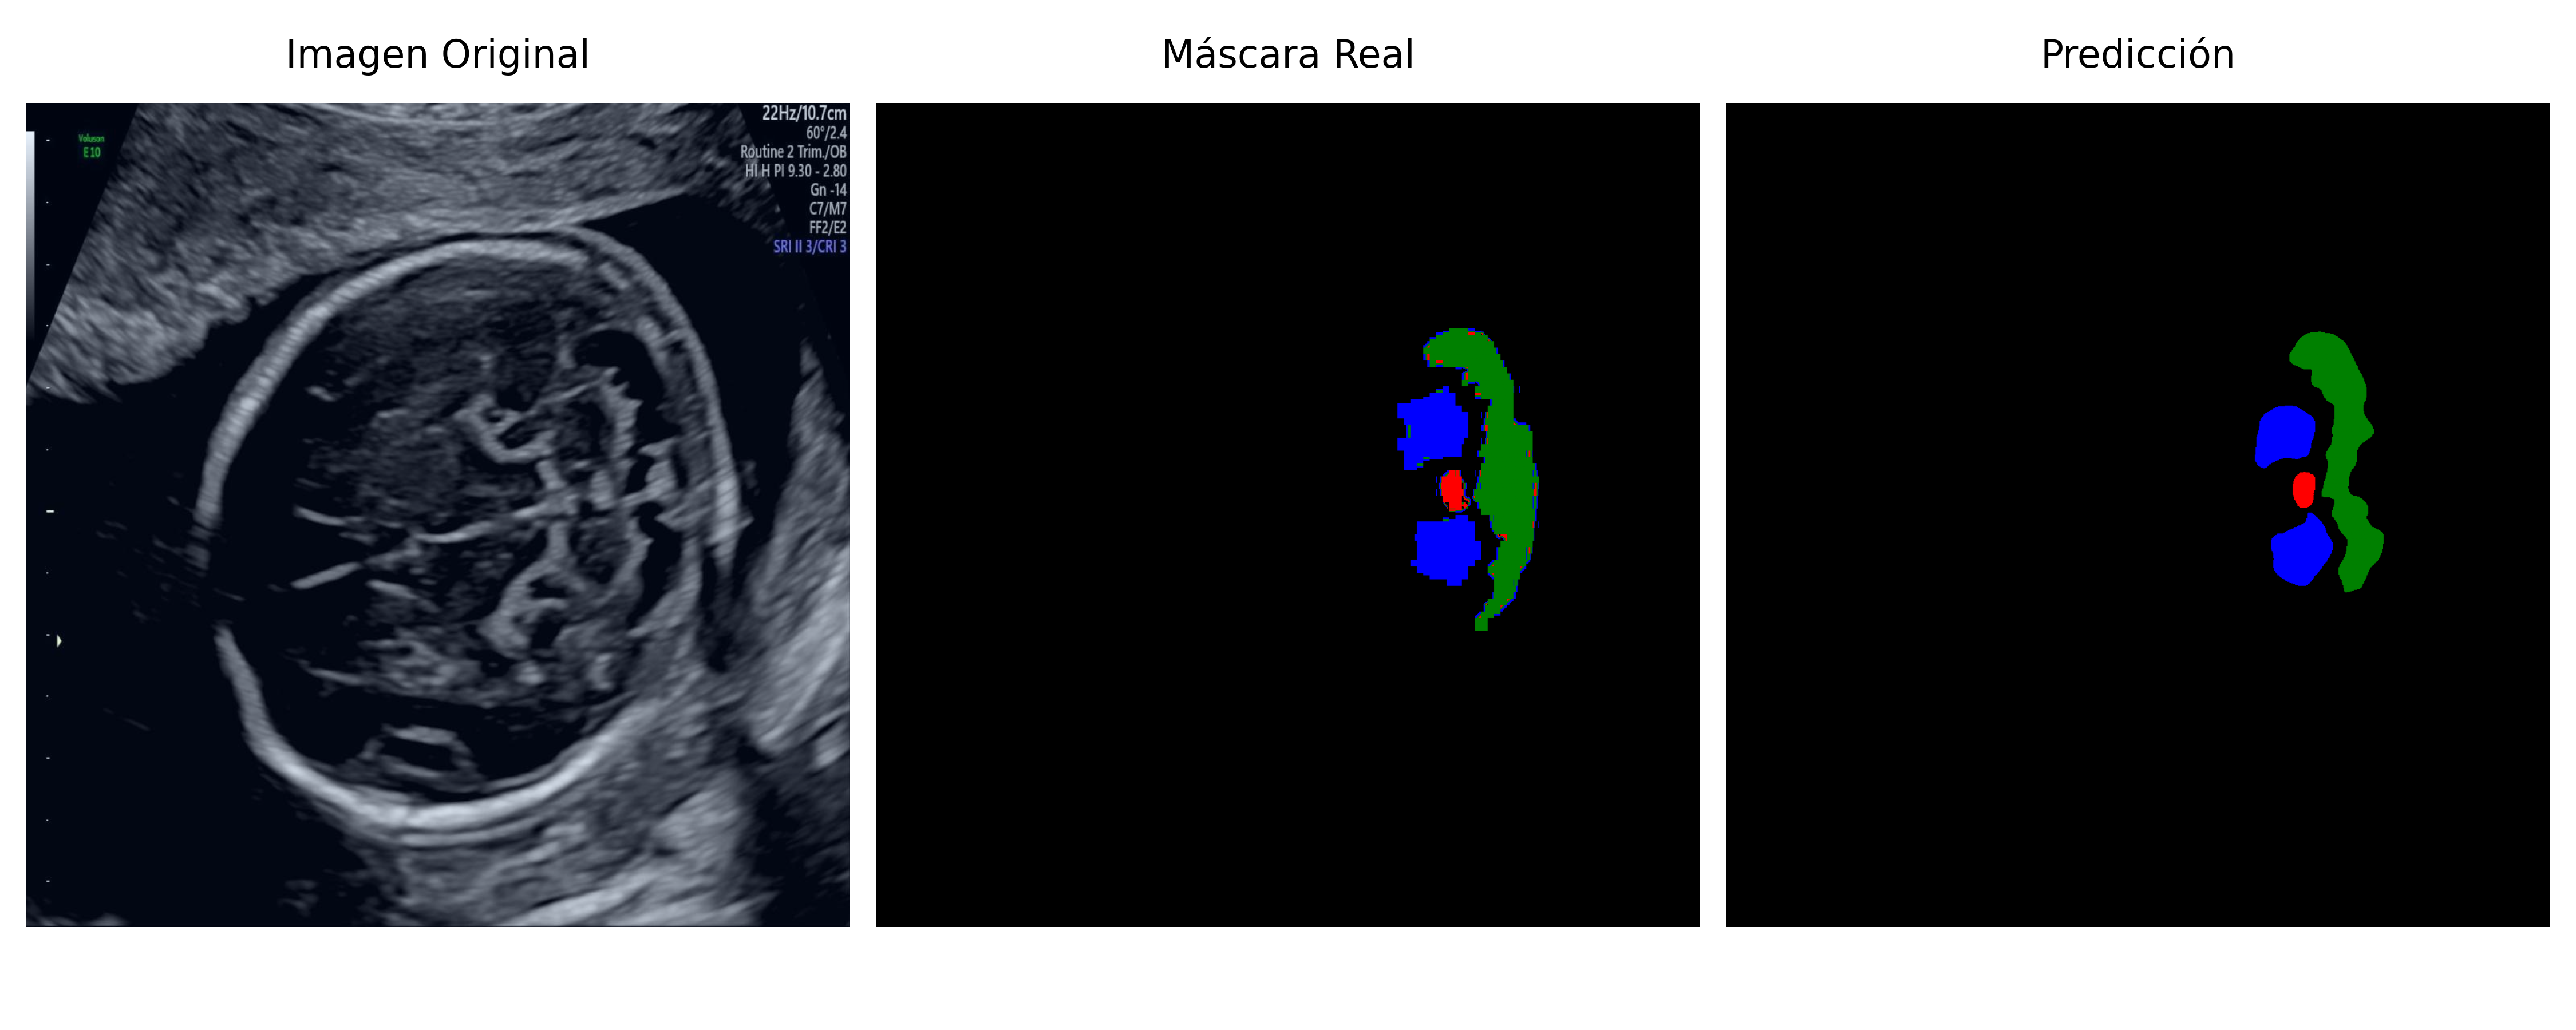
\includegraphics[width=1\textwidth]{img/image2_unet.png}
    \caption{Ejemplo adicional de segmentación con U-Net.}
    \label{fig:comparacion_unet2}
\end{figure}

\begin{figure}[h]
    \centering
    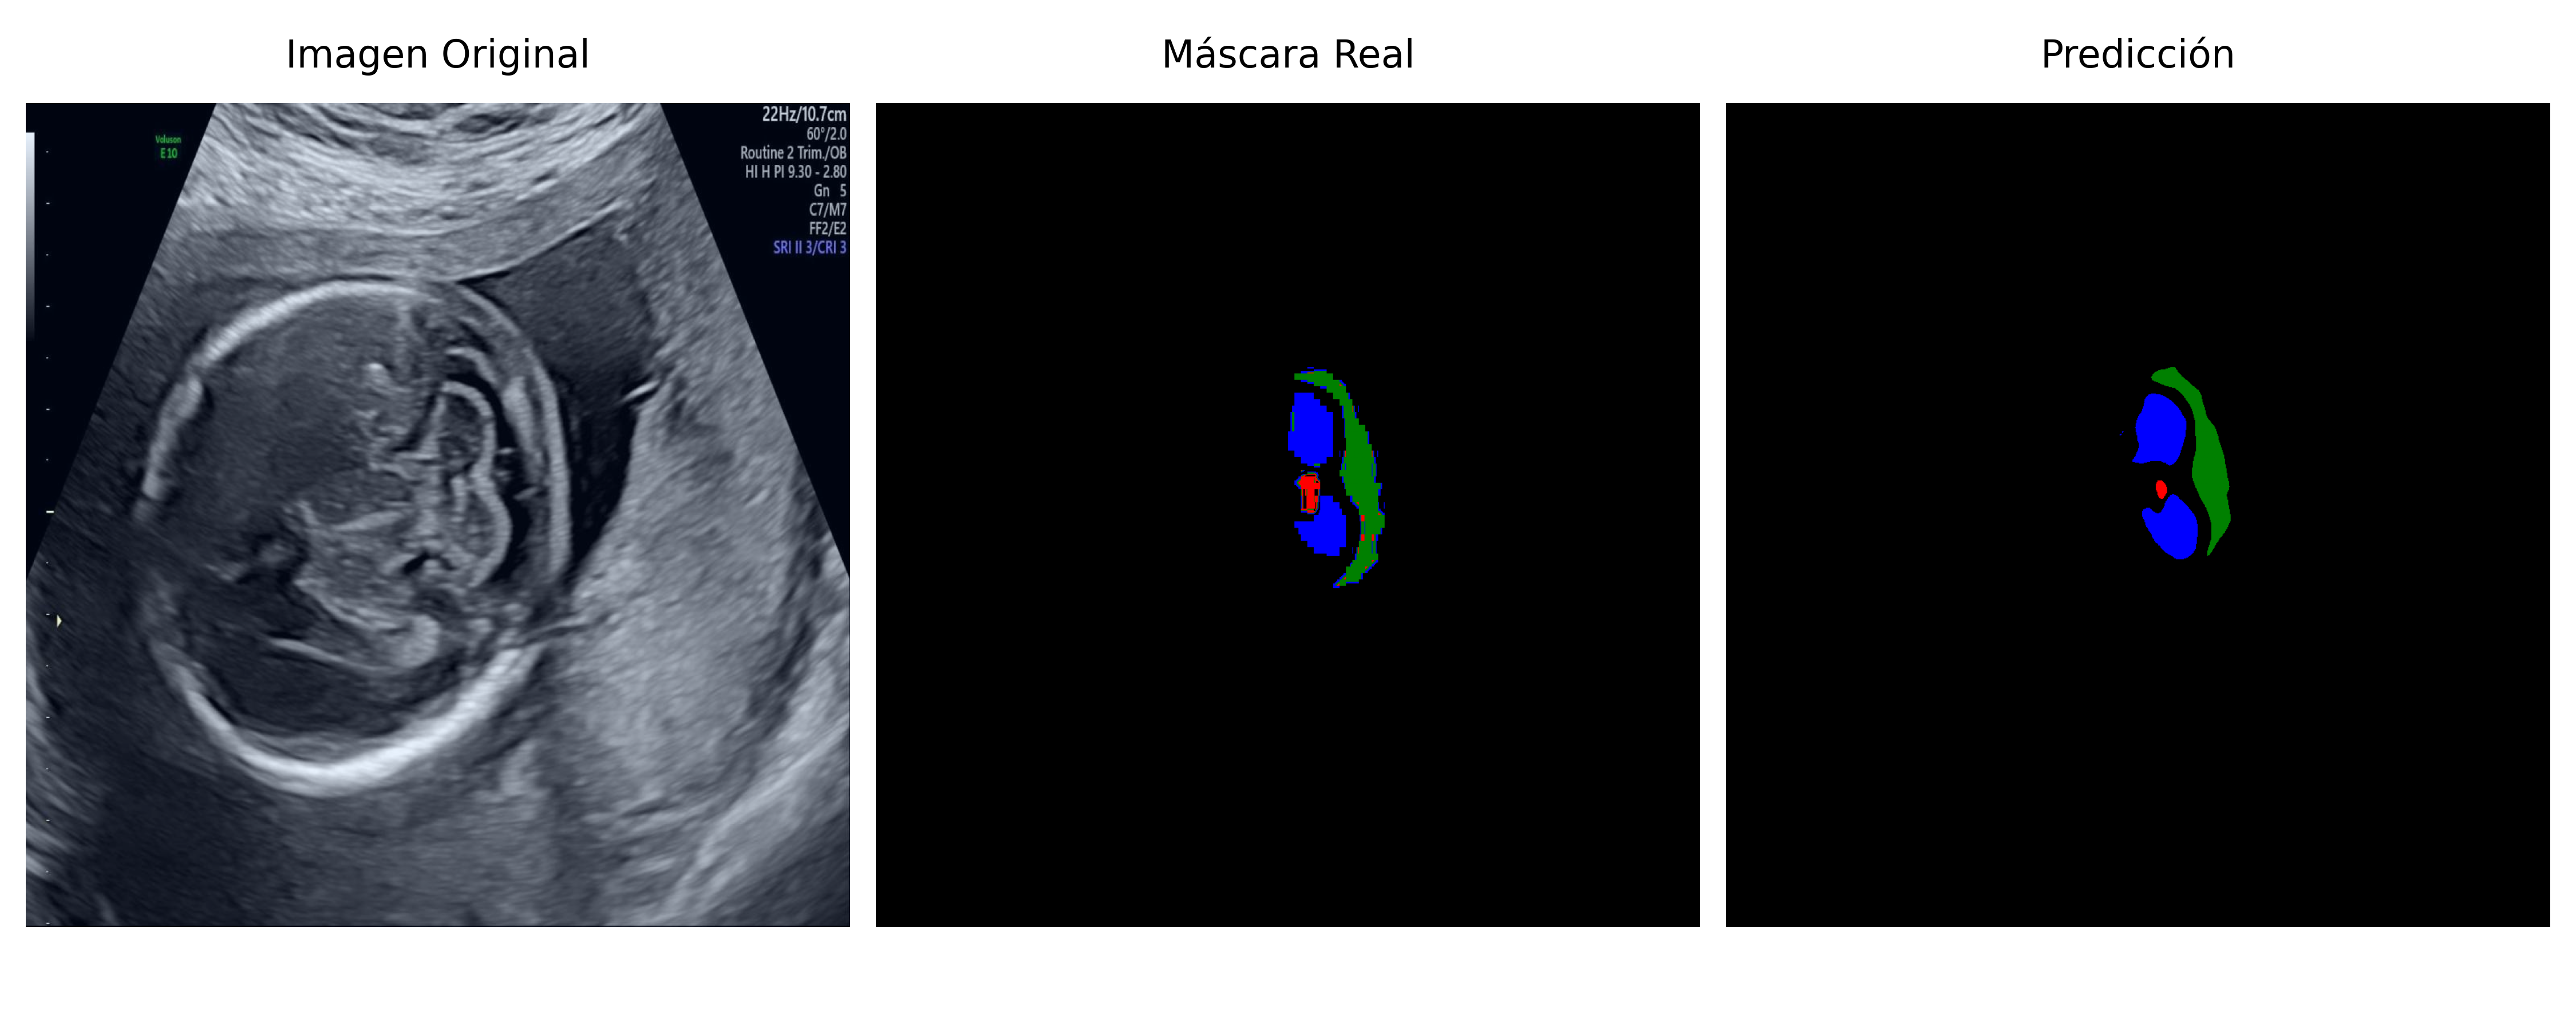
\includegraphics[width=1\textwidth]{img/image3_unet.png}
    \caption{Segunda visualización de resultados con U-Net.}
    \label{fig:comparacion_unet3}
\end{figure}

\begin{figure}[h]
    \centering
    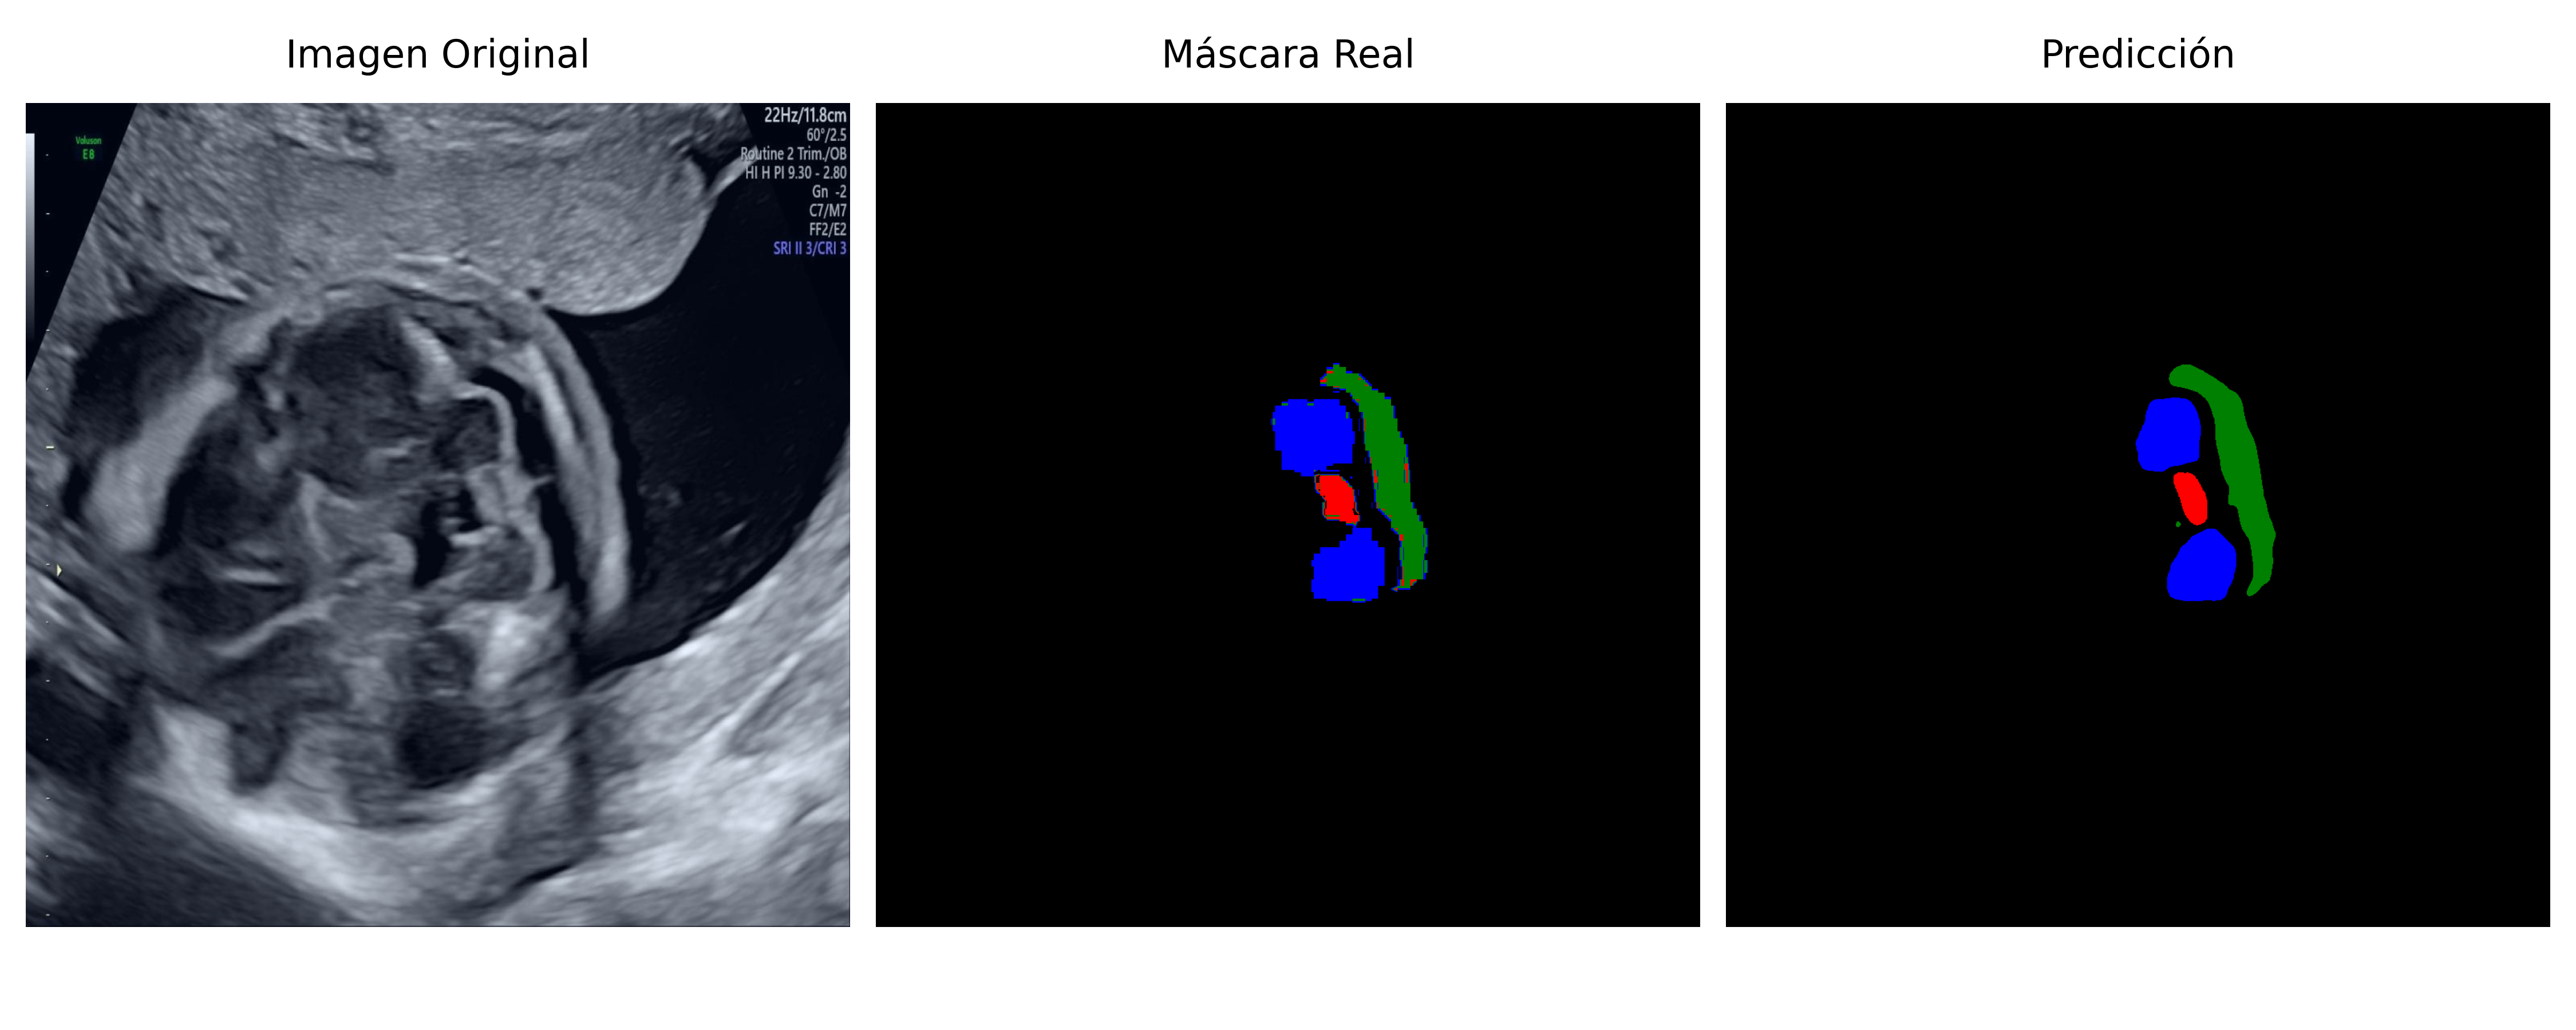
\includegraphics[width=1\textwidth]{img/image4_unet.png}
    \caption{Tercer ejemplo de segmentación con U-Net.}
    \label{fig:comparacion_unet4}
\end{figure}

Como parte del resultado final del proyecto, se desarrolló una interfaz que permite al personal clínico cargar imágenes de ecografía, visualizar las segmentaciones generadas por el modelo, consultar la máscara \textit{ground truth} cuando está disponible y generar automáticamente informes en formato PDF.

Esta interfaz fue desarrollada inicialmente en \textit{Streamlit} y posteriormente desplegada en la nube mediante \textit{Streamlit Community Cloud}, permitiendo su uso sin necesidad de instalaciones locales. La herramienta está disponible en el siguiente enlace: \url{https://fetalbrainsegmentation.streamlit.app/}.

Las Figuras \ref{fig:subir_imagenG}, \ref{fig:visualizar_segmentaciónG}, \ref{fig:generar_informeG} muestran capturas de pantalla representativas de la aplicación.

\begin{figure}[h]
    \centering
    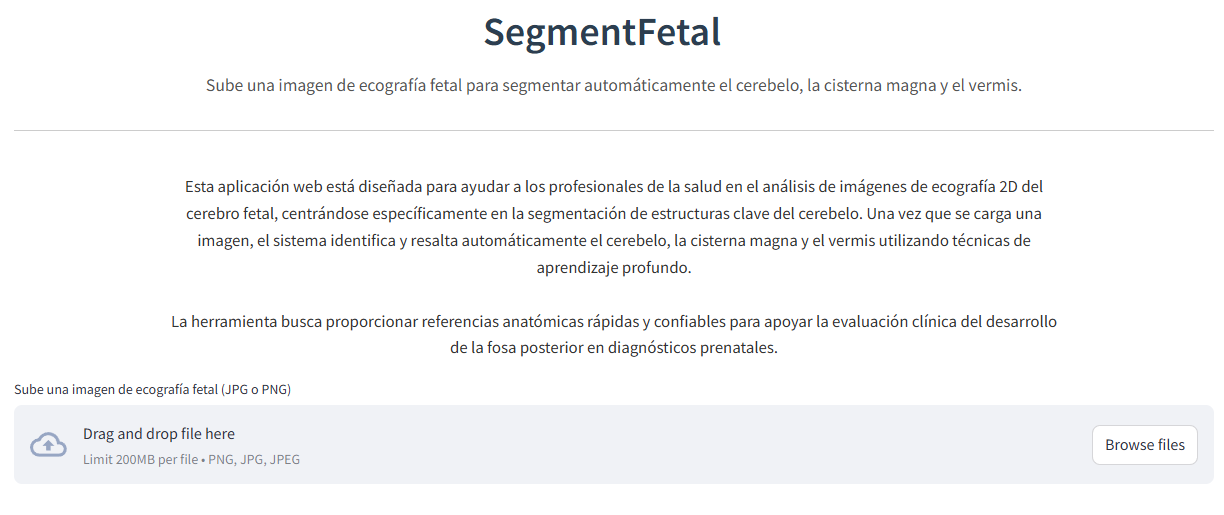
\includegraphics[width=1\textwidth]{img/interfaz_subir_imagen.png}
    \caption{Cargar imagen médica.}
    \label{fig:subir_imagenG}
\end{figure}

\begin{figure}[h]
    \centering
    \includegraphics[width=1\textwidth]{img/interfaz_visualización.png}
    \caption{Visualizar segmentación automática.}
    \label{fig:visualizar_segmentaciónG}
\end{figure}

\begin{figure}[h]
    \centering
    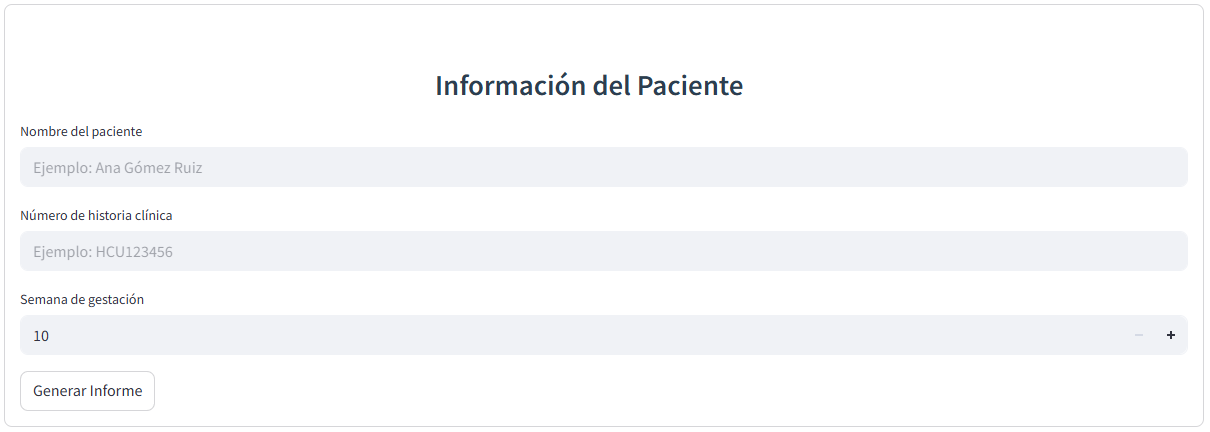
\includegraphics[width=1\textwidth]{img/interfaz_generar_informe.png}
    \caption{Generar informe.}
    \label{fig:generar_informeG}
\end{figure}

\apendice{Anexo de sostenibilización curricular}

\section{Introducción}
El proyecto se ha centrado en el desarrollo de una aplicación basada en inteligencia artificial para la segmentación automática de estructuras cerebrales fetales en imágenes ecográficas. Más allá del componente técnico, el proyecto ha supuesto una oportunidad para reflexionar sobre el papel que la tecnología puede desempeñar en la construcción de un sistema sanitario más justo, accesible y eficiente. En este capítulo se recoge cómo se han integrado los principios de sostenibilidad a lo largo del desarrollo del trabajo, siguiendo las directrices de la CRUE y en sintonía con los Objetivos de Desarrollo Sostenible (ODS) de la Agenda 2030.

\section{Tecnología para el bien común (ODS 3 y ODS 10)}
Uno de los pilares fundamentales de este proyecto ha sido la voluntad de mejorar la atención sanitaria mediante soluciones tecnológicas accesibles. Al desarrollar una aplicación capaz de asistir en el diagnóstico prenatal, se contribuye directamente al ODS 3: Salud y Bienestar, facilitando la detección precoz de posibles alteraciones en el desarrollo fetal. Esta detección, además, puede realizarse sin necesidad de equipamiento costoso o intervenciones invasivas, lo que la hace especialmente útil en contextos clínicos con recursos limitados.

Además, se promueve una sanidad más equitativa (ODS 10: Reducción de las desigualdades), ya que la inteligencia artificial puede reducir la variabilidad diagnóstica entre profesionales, democratizando el acceso a una segunda opinión médica automatizada, especialmente en zonas rurales o con escasez de especialistas.
\section{Eficiencia y sostenibilidad tecnológica (ODS 9 y ODS 12)}
Durante el desarrollo del proyecto, se han tomado decisiones orientadas a minimizar el consumo de recursos computacionales. Por ejemplo, el uso de técnicas como el early stopping permiten reducir el tiempo de entrenamiento y el uso de energía. Estas prácticas están alineadas con el ODS 12: Producción y consumo responsables y el ODS 9: Industria, innovación o infraestructura, promoviendo soluciones digitales sostenibles y eficientes.

Asimismo, se ha priorizado el uso de herramientas y librerías de código abierto (como PyTorch Lightning, OpenCV, Streamlit y COCO) fomentando la reutilización de software y reduciendo la dependencia de licencias comerciales, lo que además refuerza la accesibilidad para futuros desarrolladores o centros hospitalarios con recursos limitados.

\section{Educación, responsabilidad ética y desarrollo profesional (ODS 4 y ODS 17)}
Este trabajo me ha ayudado a desarrollar una conciencia ética respecto al uso de los datos médicos. He trabajado con conjuntos de datos sensibles, por lo que he tomado medidas para preservar la anonimización y asegurar un uso responsable de la información. Esta reflexión está directamente relacionada con el ODS 4: Educación de calidad, ya que he podido aplicar de forma transversal los principios éticos y de responsabilidad social aprendidos a lo largo del grado.

Además, al integrar el proyecto dentro de un ecosistema de trabajo reproducible, documentado y abierto a colaboraciones, se favorece el desarrollo de alianzas interdisciplinares (ODS 17: Alianzas para lograr los objetivos). La interfaz que he desarrollado de software contribuye a una integración real de la tecnología en el entorno médico.

\section{Conclusión}
A través de este trabajo, he podido comprobar que la sostenibilidad no se limita al ámbito ambiental, sino que también implica compromisos sociales, éticos y educativos. Integrar estos principios en un proyecto técnico ha supuesto un desafío enriquecedor y he reforzado mi convicción de que, como futura profesional de la ingeniería de la Salud, tengo la responsabilidad de aplicar mis conocimientos al servicio de una sociedad más justa, inclusiva y sostenible. En este sentido, el proyecto representa una pequeña aportación al compromiso colectivo con los ODS y con un desarrollo tecnológico humano.




\bibliographystyle{ieeetr}
\bibliography{bibliografiaAnexos}

\end{document}
